\documentclass{article}

\usepackage{fontspec}
\usepackage{array}
\usepackage{graphicx}
\usepackage{amsmath}
\usepackage{geometry}
\usepackage{amsmath}
\usepackage{algorithm}
\usepackage{algpseudocode}
\usepackage{amssymb}

\usepackage{subcaption} 
\newcommand{\myimagepath}{/Users/davidhodgson/Dropbox/Mac (3)/Documents/research/Rpackages/rjmc/}


\geometry{
    top=1in,
    bottom=1in,
    left=1in,
    right=1in,
}
\setmainfont{Avenir} 
\newcolumntype{M}[1]{>{\centering\arraybackslash}m{#1}}

%
\title{Modelling serological data using reversible jump Markov chain Monte Carlo}
\author{David Hodgson, James Hay(?) and Adam Kucharski\\\small Center of Mathematical Modelling of Infectious Diseases\\\small London School of Hygiene and Tropical Medicine}
\date{\today}

\begin{document}

\maketitle

\section{Overview of serological modelling}

\subsection{Introduction}

\paragraph{}Serological samples can be analysed to detect the presence of biomarkers made in response to an infection long after the infection has cleared.\cite{Cutts2016} Therefore, analysing serological samples allows researchers and healthcare professionals to deduce crucial information about the epidemiology of a pathogen at the individual and population level, which active virological surveillance systems may otherwise miss.

\paragraph{}On the individual level, after measuring antibodies to a specific pathogen, infection is usually inferred using either i) an antibody threshold level (seropositive) or ii) a threshold fold-rise between a pair of samples (seroconverted).\cite{Haselbeck2022} Often, researchers are interested in understanding how seropositivity and seroconversion rates change according to controlled host factors, such as age, XXXX etc.\cite{} On the population level, serological samples which are representative of a population (e.g. cross-sectional samples) can be used to estimate the prevalence of infectious diseases (seroprevalence) and determine how seroprevalence changes over time according to host factors.\cite{} Estimates of seropositivity, seroconversion, and seroprevalence can help the understanding of the immune system's ability to combat various pathogens, aid in developing new targeted intervention programmes and provide insights into the transmission dynamics of infectious diseases. The methods used to analyse serological samples to inform epidemiology and public health have been termed 'serodynamics' and have recently been reviewed. \cite{Hay2023}

\paragraph{}Serological samples play an increasingly important role in public health efforts to combat and control infectious diseases.\cite{Haselbeck2022;Metcalfe2015} However, inferring infection through seropositivity or seroconversion requires deriving an absolute or relative threshold hold value, and these are often determined by rule-of-thumb heuristics (e.g. flu, 4-fold-rise for conversion, titre of 1:40 HAI for seropositivity).\cite{Xu2020} However, antibody responses vary greatly between individuals for many pathogens; therefore, relying on these heuristics to determine infections in serology studies can lead to incorrect infection status being inferred, potentially leading to biased estimates.\cite{Chan2021;Cauchesmez2021} Consequently, a better understanding of the kinetics of antibody trajectories post-vaccination and infection can help establish and ascertain the accuracy of existing heuristics and be used to more accurately infer infection status.

\subsection{Antibody kinetics}

\paragraph{}Modeling antibody kinetics involves using mathematical and statistical techniques to simulate the trajectories of antibodies in response to an infection or vaccination. \cite{Hay2023} Typically, this involves the use of mathematical equations and statistical methods to describe the time-dependent changes in antibody levels within an individual or a population. This process is essential for understanding how antibody levels evolve and, therefore, potentially provide protection against infectious diseases. Various functional forms have been used to model the individual-level kinetics of antibody trajectories,\cite{} typically it follows a three-stage process:

\begin{itemize}
\item \textit{Initial} Response: The trajectories often start by capturing the initial antibody response to a pathogen or vaccine. This phase is characterized by a rapid increase in antibody levels as the immune system recognizes and mounts a defence against the antigen.

\item \textit{Peak Antibody Level}: The trajectories then rise to apeak antibody level, which is the highest concentration of antibodies reached during the immune response. This peak can vary depending on factors like the strength of the immune response and the nature of the antigen.

\item \textit{Decay Phase}: After the peak, there is a decline in antibody levels. Antibodies have a finite lifespan in the bloodstream, and their concentration gradually decreases as the pathogen is cleared or the vaccine antigen wanes. Often antibodies secreted from now-establish long-lived plasma cells, the decay phase trajectories fall to a set point titre.\cite{srivasta}
\end{itemize}


\paragraph{}Modeling antibody kinetics provides several important benefits. First, by understanding the rate of antibody decline, models can estimate how long an individual's immunity is likely to last after infection or vaccination. This information is critical for designing vaccination schedules and determining the need for booster shots and permits the creation of better heuristics for determining infections using serology. Kinetics are also useful for optimizing vaccination strategies and can help identify the optimal timing and frequency of booster vaccinations to maintain protective antibody levels within a population. This is especially important for vaccine-preventable diseases with varying immunity levels such as influenza and COVID-19.

\subsection{Correlates of protection}
\paragraph{} A correlate of protection is an immune function or biomarker that correlates with and or may be biologically responsible for protection against infection or disease. Correlates of protection have been established for influenza, Hepatitis A and B, Measles, Polio, Rabies, Yellow fever and more.\cite{Plotkin} Correlates of protection help researchers understand the specific immune responses needed to prevent or control an infectious disease. This knowledge is pivotal in designing and optimizing vaccines to induce the required immune response effectively.\cite{}

\paragraph{}Correlates of protection can be established by i) comparing the immune response of those protected by the vaccine with so-called ‘breakthrough cases’, where clinical disease manifests despite prior vaccination and ii) human challange studies.\cite{} 

\paragraph{}A natural biomarker for a correlate of protection from infection is the amount of neutralising antibodies in the serum as this measures a serum's ability to prevent viral particles from infecting vulnerable cells. Therefore, those with high levels of neutralising antibodies could abort an infection by neutralising viral particles in-host even if exposed to a virus. Determining the immonlogical profiels of individuals are exposed to an infection but manage to abort it due is crucial for determining a universal correlate of protection. Usually, these individuals are identified through challenge studies, allowing for a direct evaluation of correlates of protection, however these studies are expensive, difficult to run, can only be performed on healthy individuals, and are only possible for pathogens with general pathogenesis.

\paragraph{}Using serological samples to establish a correlate of protection would solve the aforementioned problems with challenge studies as they are cheaper to conduct and less invasive. However, determining correlates of protection through serological studies is challenging to establish because those who have been exposed but then experience an abortive infection generally leave no measurable antibody imprint. Therefore serological studies can be augmented with either immunological profiling to determine other immunological biomarkers that indicate abortive infection\cite{} or include intensive contact tracing with the serological studies to determine exposure rates between individuals\cite{}. Augmented serological studies with these additional increase the complexity and cost of a study and, therefore, are not feasible in many settings.


\subsection{Overview of modelling framework}

\paragraph{}If antibody trajectories are known for every individual throughout a study and the time of infection is known, then we can determine the probability of infection for a given titre value. Though not strictly a correlate of protection, as we do not know whether non-infected individuals have been exposed, this can be useful for determining associations between infected and non-infected individuals for a given population. However, relying on this sample to establish correlates of protection can lead to bias estimates XXX. 

\paragraph{}In this document, we present a single modelling framework which takes individual-level serological sample data and uses changes in antibody titres over time to determine i) which individuals have seroconverted throughout the study, ii) subsequent antibody kinetics of these infection individuals, iii) which individuals are exposed throughout the study, and iv) the correlate of protection preventing exposed individuals from becoming infected. Though the infection and exposure status is often unknown for most individuals in a serological study, we find that by using broad, biologically-informed mechanistic forms for the antibody kinetics and correlation of protection, the infection and exposure status of individuals and the popoulation are recoverable through the interdependencies of mechanisms i)–iv) within a Bayesian probabilistic framework. 




\newpage
\section{Simulated serological data from \texttt{serosim}}

\begin{figure}[h]
    \centering
    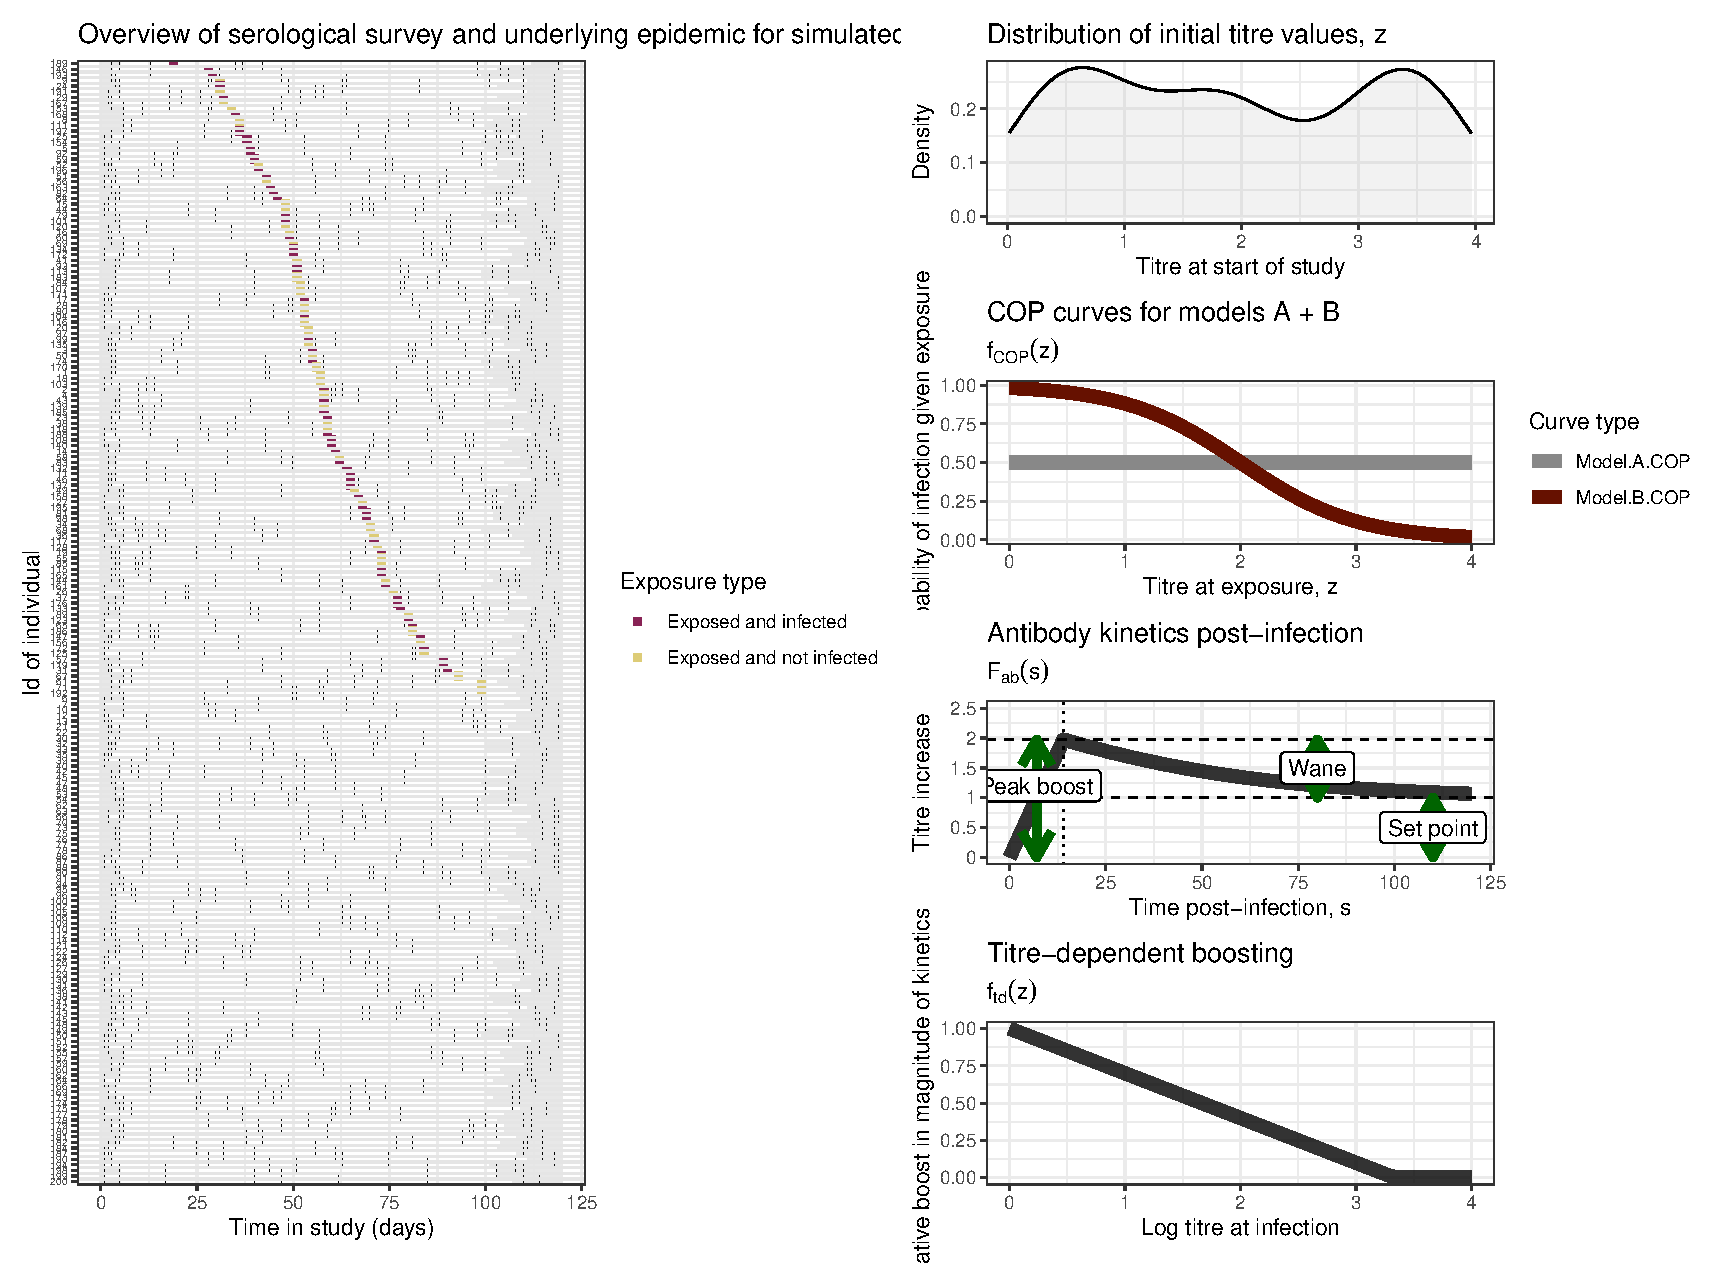
\includegraphics[width=1\textwidth]{\myimagepath/outputs/sim_data/summary_fig_A_CES.pdf}     \caption{Schematics showing the simulated data structure from \texttt{serosim}[ref]}
    \label{fig:sim_A}
\end{figure}

\paragraph{}To demonstrate the effectiveness of our modelling framework, we simulate serological data using the \texttt{serosim}[ref] R package to demonstrate its capabilities at simulation recovery. We simulate continuous epidemic serosurveillence (CES) cohort data, which represents a study in which individuals are followed over a period spanning an epidemic wave and bled at multiple random time points throughout. The simulated data includes $ M = 200$ individuals with serological samples taken within the first seven days of the study's starting and a sample within the last seven days of the study's ending. These individuals also had three samples taken randomly throughout the study (over the 120-day epidemic wave). Each individual has a 60\% chance of exposure to the virus over the study timeframe and can have a maximum of one exposure. To model an even epidemic peak, we simulate the exposure time for each individual from a normal distribution, $N(60, 20)$ days.% A figure showing the timing of the bleeds, infections and exposures for each individual is given in Figure ~\ref{fig:sim_A}.

\paragraph{}We define a correlate of protection as the probability of infection given a titre value at exposure. Two sets of data are simulated with two different correlates of protection; one is uniform at 50\% for all titres at exposure (COP model A) and thus represents no titre-dependent protection correlation. The second follows a logistic distribution (COP model B) of the form:

\begin{equation}
\label{eq_cop}
f_{cop}(x, \beta_0, \beta_1) = \frac{1}{1 + \exp(- (\beta_0 + \beta_1x))}
\end{equation}

where $\beta_0 = 2$ and $\beta_1 = 2$ in the simulated data and $x$ is the titre value at exposure. This represents a pathogen for which higher antibody titres are associated with higher levels of protection from infection. Note in this data we assume antibody trajectories remain constant until the timing of infection, such $f_{cop}(X_{j, t}, \beta_0, \beta_1) = f_{cop}(Z^0_{j}, \beta_0, \beta_1)$ where $Z^0_{j}$ is the antibody titre of an individual at their first bleed at the start of the study.

\paragraph{}Following infection, the antibody kinetics are assumed to follow a linear rise to a peak at 14 days, followed by an exponential decay to a set-point value as defined in X[ref]. The formula for this biphasic trajectory is given by Equation~\ref{eq_ab}.

\begin{equation}
\label{eq_ab}
f^1_{ab}(s, a, b, c) =
\begin{cases}
  \ln(\exp(a) + \exp(b)) / 14, & \text{if }s \leq 14 \\
  \ln(\exp(a) \exp(-(b/10)(t - 14)) + \exp(c)), &\text{if } s > 14
\end{cases}
\end{equation}

where $a = 1.5$, $b = 2$, and $c = 1$ are values in the simulated data (Figure) and $s$ is the number of days post infection. We also assume that the magnitude of these dynamics depends on pre-existing titre values, with higher pre-existing values seeing attenuated dynamics relative to lower pre-existing tire values. The titre dependent boosting is assumed to follow a linear decay truncated at 0, that is, given a titre value $z$, $f^2_{ab}(Z_j^0, \alpha) = \max(1 - \alpha z, 0)$. where $\alpha = 0.3$ in the simulated data. Therefore, the model estimated titre value at time $t$ for individual $j$, given time $s$ since infection with a titre value at infection of $Z_{j}^0$, is given by;  

\begin{equation}
\label{eq_ab2}
f_{ab}(s, Z^0_{j}, a, b, c, \alpha) = f^1_{ab}(s, a, b, c)f^2_{ab}(Z^0_{j}, \alpha) 
\end{equation}


\begin{figure}[h]
    \centering
    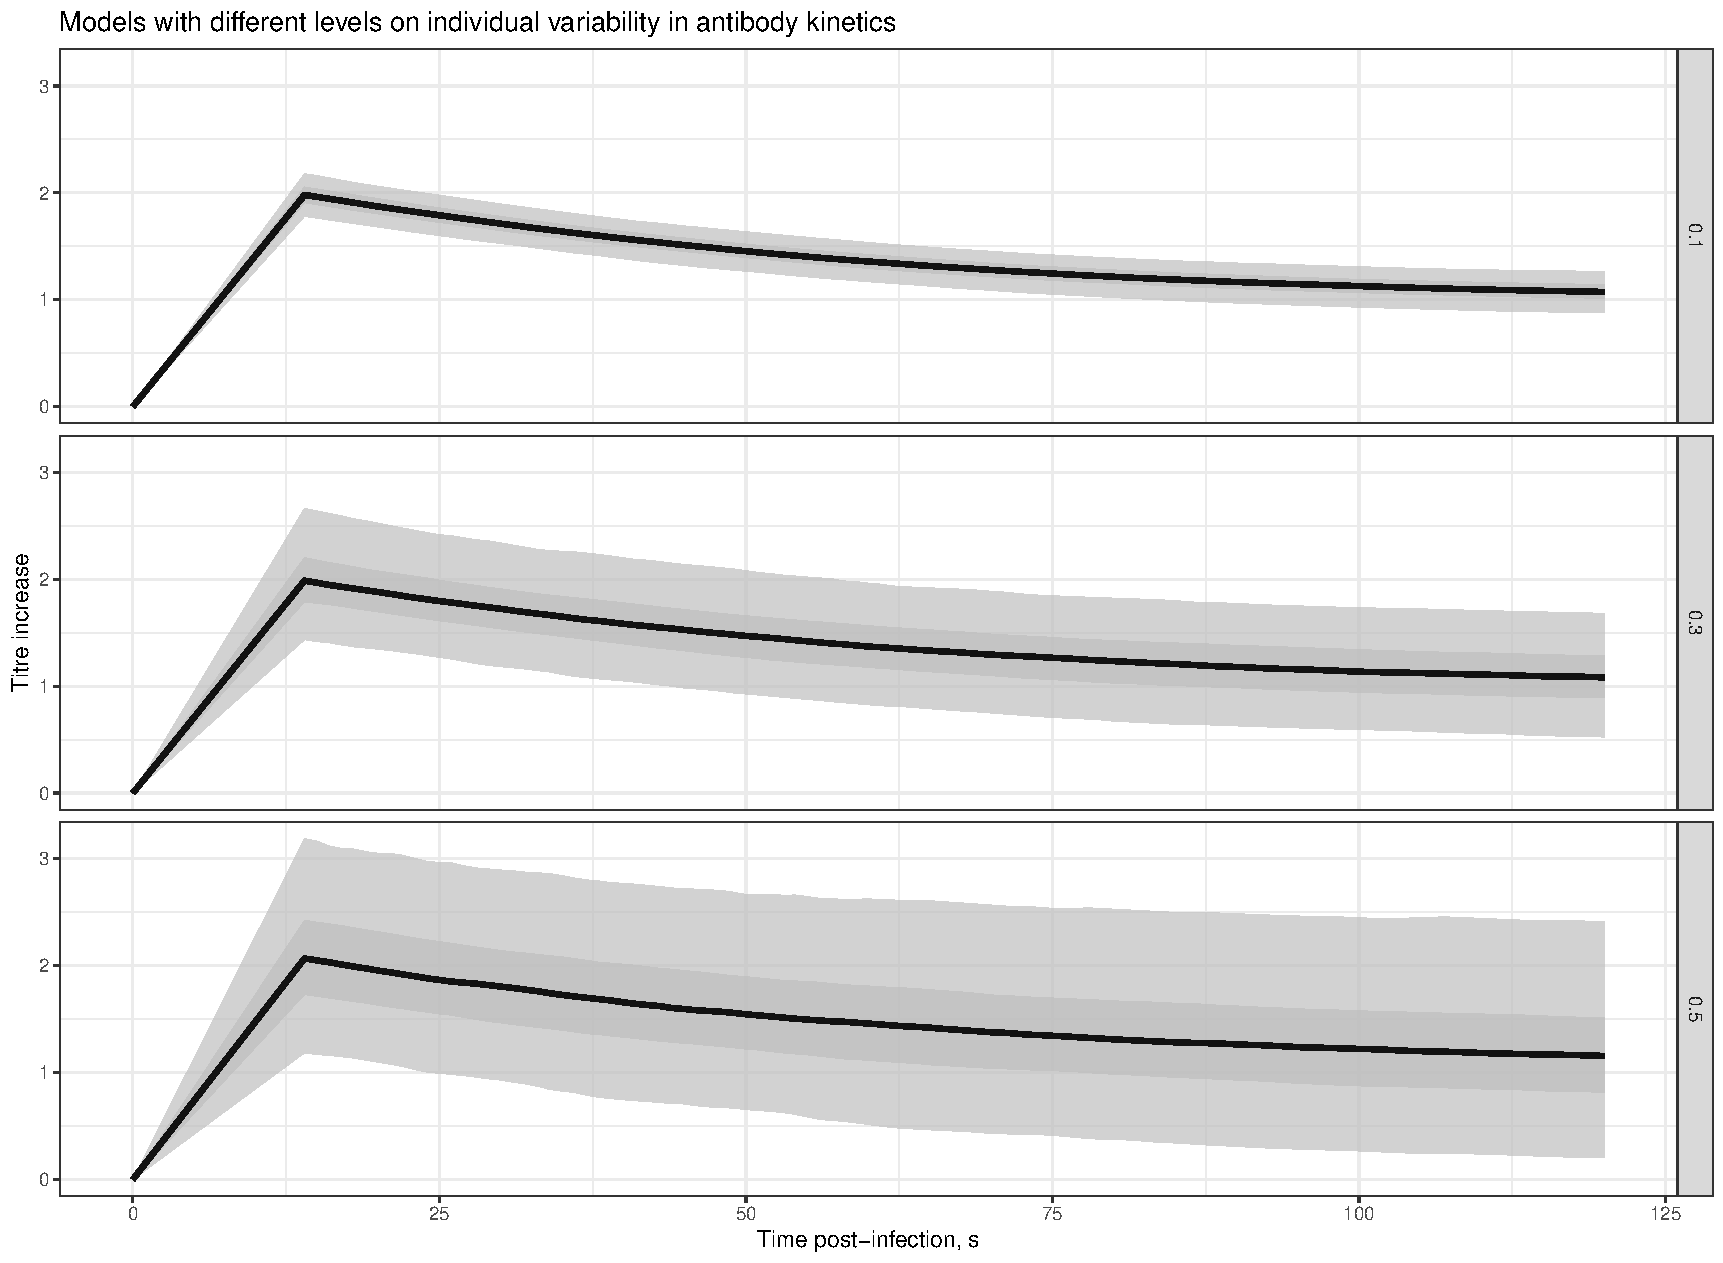
\includegraphics[width=1\textwidth]{\myimagepath/outputs/sim_data/summary_fig_B_CES.pdf}     \caption{Schematics showing three levels of individual-level uncertainty and the impact on the variability of antibody kinetics.   }
    \label{fig:sim_B}
\end{figure}



\paragraph{}To model heterogeneity in individual-level antibody kinetics, we simulate $a, b, c$, and $\alpha$ from normal distributions where the mean $\mu$ is their simulated values and the standard deviation given by $\mu\sigma^*$. We simulate three levels of uncertainty for $\sigma^* = \{0.1, 0.3, 0.5\}$, for both of the COP models, giving six simulated datasets in total. A schematic showing how these levels of uncertainty influence the variability of the antibody kinetics trajectories is shown in Figure~\ref{fig:sim_B}. We will fit the to-be-described methods to these datasets and explore how the correlation of protection and level of variability in antibody kinetics impacts the framework's ability to recover simulated data. 



We note that the simulated data for the correlate of the protection doesn't not exact match the functional form chosen when it is inferred from the infected population~\ref{}

\begin{figure}[h]
    \centering
    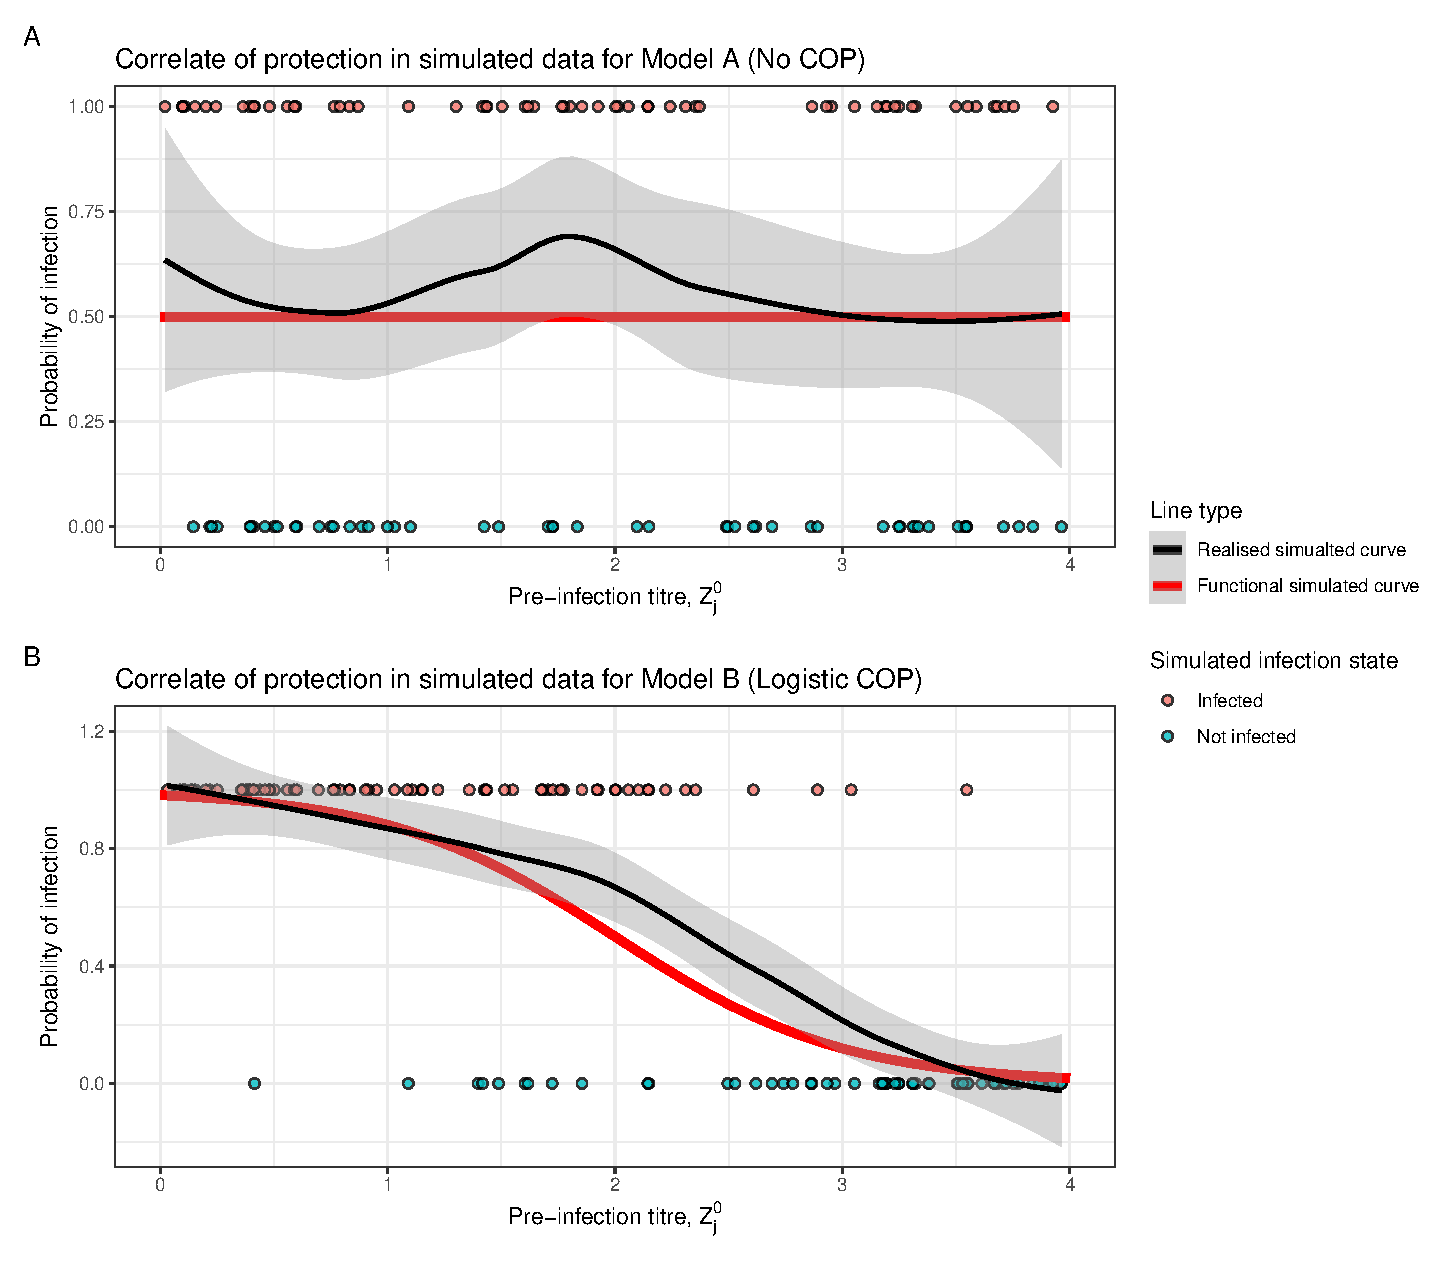
\includegraphics[width=1\textwidth]{\myimagepath/outputs/sim_data/summary_fig_C_CES.pdf}     \caption{Schematics showing the difference between the functional form chosen to simulate the COP and the recovered COP from the exposed individuals.   }
    \label{fig:sim_C}
\end{figure}



\newpage
\newpage

\section{Inference with known exposure status}

\paragraph{}Before we look at the reversible-jump mcmc algorithm (RJMCMC), we will show simulation recovery in a simplified framework where we assume the exposure status of every individual (represented by vector $\mathbf{E}$) and exposure time (represented by vector $\mathbf{E^\tau}$) is known. Though knowing this information is rarely feasible in practice, working through this example will help explain how the inference on the fitted parameters $\theta$ and infection state $\mathbf{I}$ work without needing to describe the more complex inference using RJMCMC. 

\subsection{Mathematical representation of framework}

\paragraph{}Let the binary vector $\mathbf{E} = \{ E_1, E_2, \dots, E_M\}$, represent the exposure status of each individual $j$ where $E_j = 0$ is not exposed and $E_j = 1$ is exposed and let $n_\mathbf{E} = \sum_{j = 1}^ME_j$ be the number of exposed individuals. Then, let the vectors $\mathbf{E}^\tau = \{E_1^\tau, E_2^\tau, \dots, E^\tau_{n_\mathbf{E}}\}$ and $\mathbf{I} = \{I_1, I_2^, \dots, I_{n_\mathbf{E}}\}$ be the timing of the exposure and the infection state respectively for each individual which is exposed. The infection state is a binary vector where $E_j = 0$ is not infected, and $I_j = 1$ is infected. Let $Z_{j, t} \in \mathbf{Z}$ represent the dataset of titre values for individual $j$ and at time $t$. 

\paragraph{}We define several functions to help us calculate the likelihood of our model. First, we assume that the model predicted antibody titre at time $t$ in the study ($X_{j.t}$) can be derived given the infection status $I_j$ and timing of exposure $E_j^\tau$. If a person is not infected, their starting titre value ($Z^0_i$) remains unchanged from the start of the study. If the person is infected, their titre remains unchanged until the point of infection, at which point they follow the dynamics highlighted in Equation~\ref{eq_ab2}. The deterministic function for calculating $X_{j,t}$ value is given by

\begin{equation}
\label{eq:ll_abkin}
X_{j,t}  = F_{ab}( I_j,  E_j^\tau, \theta_{ab}, Z^0_j) = 
	\begin{cases}
	Z^0_j + f_{ab}(t - E_j^\tau, \theta_{ab}, Z^0_j),  & \text{If $I_j = 1$, $E_j = 1$, and $t > E_j^\tau$} \\
	Z^0_j, & \text{Otherwise} \\ 
	\end{cases}
\end{equation}

Where $\theta_{ab} = \{a, b, c, \alpha\}$. Second, we define a likelihood function for the correlation of protection. For an individual $j$, with $E_j = 1$, the correlate of protection given exposure at time $t$ with titre value $X_{j, t}$, given by a Bernoulli distribution with the probability is given by Equation~\ref{eq_cop}. The PDF of this likelihood is given by Equation~\ref{eq:ll_cop}.

\begin{equation}
\label{eq:ll_cop}
P_{cop}(I_j \mid Z_{j}^0, \theta_{cop} ) =  f_{cop}(Z_{j}^0,  \theta_{cop})^{I_j}(1- f_{cop}(Z_{j}^0,  \theta_{cop} ))^{1-I_j}
\end{equation}

\paragraph{}$\theta_{cop} = \{\beta_0, \beta_1\}$. Finally, we define an observational model to capture variability between hosts and measurement error. Given $X_{j.t}$ and the serological antibody data at the same time point is given by $Z_{j, t}$, we assume the measurement error follows a normal distribution with a PDF given by Equation~\ref{eq:ll_obs}.

\begin{equation}
\label{eq:ll_obs}
P_{obs}(Z_{j,t} \mid X_{j,t}, \sigma) = \frac{1}{\sigma \sqrt{2\pi}} \, e^{-\left(\frac{(Z_{j,t} - X_{j,t})^2}{2\sigma^2}\right)}
\end{equation}

Let $\theta = \{a, b, c, \alpha, \beta_0, \beta_1, \sigma\}$ be the set of continuous parameters which are to be fitted in the model. 

\subsection{Posterior distribution via Bayes rule}

We have two different likelihoods depending on whether an individual is exposed ($E_i = 1$) or not ($E_i = 0$).

\subsubsection{Likelihood for an non exposed individual $E_j = 0$} 
In this case, the value of the timing of exposure and infection status is not applicable and thus not inferred. The likelihood for individual $j$ with serological samples taken at times $t\in T_j$ is therefore equivalent to:
\begin{equation}
L_{E_j = 0}(Z_{j}| \theta) = \prod_{t \in T_j}P_{obs}(Z_{j,t}|Z^0_{j}, \sigma)
\end{equation}
as $X_{i.t} = Z^0_{i}$ for all $t$.


\subsubsection{Likelihood for an exposed individual $E_j = 1$}
In this case, the infectious status is determined by the correlation of the protection likelihood ($P_{cop}$) and the antibody kinetics. The likelihood for this individual with serological samples taken at times $t\in T_j$ and infection time $E^\tau_j$ is therefore equivalent to:

\begin{equation}
L_{E_j = 1}(Z_{j}| I_j, \theta) = \prod_{t \in T_j}P_{obs}(Z_{j,t}| X_{j,t}, \sigma)P_{cop}(I_j \mid Z_{j}^0, \theta_{cop})
\end{equation}

where $X_{j,t} = F_{ab}( I_j,  E_j^\tau, \theta_{ab}, Z^0_j)$.


\subsubsection{Total likelihood}

If $\mathbf{E_0}$ and $\mathbf{E_1}$ are vectors representing the set of individuals who are not exposed and exposed, respectively. Then, the total likelihood can be written 

\begin{equation}
L(\mathbf{Z} | \mathbf{I}, \theta) = \prod_{j \in \mathbf{E_0}}L_{E_j = 0}(Z_{j}| \theta) \prod_{j \in \mathbf{E_1}}L_{E_j = 1}(Z_{j}| I_j, \theta) 
\end{equation}


\subsubsection{Prior distributions}

\paragraph{}We choose prior distributions for each parameter \pi($\theta$). \textbf{Table~\ref{tab:priorsA}} summarises the chosen priors with their support. 

\begin{table}[ht]
    \centering
    \begin{tabular}{|l|l|l|}
        \hline
        \textbf{Parameter} & \textbf{Prior ($\pi$)} & \textbf{Support ($\mathcal{S}$)} \\
        \hline
        a & $\mathcal{N}(1.5, 0.5)$ & $[0.5, 4]$ \\
        \hline
        b & $\mathcal{N}(0.3, 0.05)$ & $[0, 1]$ \\
        \hline
        c & $\mathcal{U}(0, 4)$ & $[0, 4]$ \\
        \hline
        $\alpha$ & $\mathcal{U}(0, 1)$ & $[0, 1]$ \\
        \hline
        $\beta_0$ & $\mathcal{U}(-10, 10)$ & $[-10, 10]$ \\
        \hline
        $\beta_1$ & $\mathcal{U}(-10, 10)$ & $[-10, 10]$ \\
        \hline
        $\sigma$ &  $\mathcal{U}(0.01, 1)$ & $[0.01, 1]$ \\
        \hline
    \end{tabular}
    \caption{Table with Headers: Parameter, Prior, and Support}
    \label{tab:priorsA}
\end{table}

\paragraph{}We also choose the prior for the number of infections $n_\mathbf{I}$ given the number of exposed individuals $n_\mathbf{E}$ to be a Beta Binomial distribution: $\pi(\mathbf{I}) = \text{BetaBinomial}(n_\mathbf{I} | n_\mathbf{E}, 1, 1)$. Choosing this prior prevents any implicit priors that might rise from products of Bernoulli trials\ref{} as $\text{BetaBinomial}(n_\mathbf{I} | n_\mathbf{E} 1, 1) = 1 / n_\mathbf{E}$ for all $0 \leq n_\mathbf{I} \leq n_\mathbf{E}$. 


\subsubsection{Posterior distributions}

\paragraph{}Bayes' rule stipulates that the product of the prior distribution and likelihood is proportional to the posterior distribution; we can use this rule to approximate the posterior for use in the metropolis algorithm. Specifically 

\begin{equation}
\label{eq:bayes}
P(\theta, \mathbf{I} | \mathbf{Z}) \propto \mathcal{L}(\mathbf{Z} | \mathbf{I}, \theta)\pi(\theta)\pi(\mathbf{I})
\end{equation}


\subsection{Metropolis-Hasting algorithm}

\subsubsection{Overview}
\paragraph{} The Metropolis-Hastings. (MH) algorithm is a widely used method for generating samples from a target probability distribution. It falls under the broader category of Markov Chain Monte Carlo (MCMC) methods and is particularly useful when direct sampling from the desired distribution is challenging or impossible such as the likelihood described above. The Metropolis-Hastings algorithm offers a solution to this problem. It is a Markov chain-based approach that iteratively generates a sequence of samples, which eventually converge to the desired distribution. 

\paragraph{}Say we wish to sample from an intractable probability distribttion $P(x)$. The idea of the MH is to define a Markov chain so that the stationary distribution of the Markov chain is $P(x)$. That is, the resulting Markov chain from MH generates a sequence of values, denoted $\{x_1, x_2, \dots,  x_n\}$, such that as $n \rightarrow \infty$ we can guarantee that $x_i \sim P(x)$. To do this, we uniquely define the Markov chain by it's transition probabilities from $x$ to $x'$, $F(x', x)$, that must satisfy the detailed balance condition:

\begin{equation}
\label{eq:db}
F(x' \mid x)P(x)=  F(x\mid x')P(x')
\end{equation}

\paragraph{}This condition ensures that the i) probability density for the next step of the Markov chain is the same as the current density and that ii) this probability density is equal to the posterior.  To construct a transition probability which satisfies this condition, we split $P$ into a proposal distribution $q(x' | x)$ and an acceptance probability $\alpha(x, x')$:

\begin{equation}
F(x' \mid x) = q(x' | x)\alpha(x, x')
\end{equation}

A common choice for $\alpha(x, x')$ which satisfies the detailed balance condition, is the acceptance ratio given by 

\begin{equation}
\label{eq:alpha}
        \alpha(x, x') = \min\left(1, \frac{P(x')}{P(x)} \cdot \frac{Q(x \mid x')}{Q(x' \mid x)}\right)
 \end{equation}

With this, the user has a choice over the proposal distribution $Q$, which can be tailored to optimise the general algorithm given in \textbf{Algorithm~\ref{alg:metropolis_hastings}}.

\begin{algorithm}[H]
\caption{Generic Metropolis-Hastings Algorithm}
\label{alg:metropolis_hastings}
\begin{algorithmic}[1]
    \State Initialize the chain with an initial state $\theta^{(0)}$
    \For{$i = 1$ to $N$}
        \State Generate a candidate state $\theta'$ from the proposal distribution: $\theta' \sim Q(\cdot | \theta^{(i)})$
        \State Compute the acceptance ratio:
        \[
        \alpha(\theta^{(i)}, \theta') = \min\left(1, \frac{P(\theta')}{P(\theta^{(i)})} \cdot \frac{Q(\theta^{(i)} \mid \theta')}{Q(\theta' \mid \theta^{(i)})}\right)
        \]
        \State Sample $u \sim \mathcal{U}(0, 1)$
        \If{$u \leq \alpha$}
            \State Accept the candidate state: $\theta^{(i+1)} \leftarrow \theta'$
        \Else
            \State Reject the candidate state: $\theta^{(i+1)} \leftarrow \theta^{(i)}$
        \EndIf
    \EndFor
\end{algorithmic}
\end{algorithm}



\subsubsection{MH for serological inference with known exposure }

\paragraph{}In our model, we wish to sample from the posterior density function given by \textbf{Equation~\ref{eq:bayes}}, which infers $\theta$, and infectious statuses ${I_j} \in \mathbf{I}$, for $1 \leq j \leq M$ individuals. For the proposal distribution, we define independent proposal distribution for $\theta$ and $\mathbf{I}$,  such that $Q(\theta, \mathcal{I}) = q_\theta(\theta)q_I(\mathbf{I})$. At Markov chain step $i$, we have a value of the parameter space, $\theta^{(i)}$, and propose a new set of parameters $\theta'$ via the proposal distribution $\theta \sim q_\theta(\cdot | \theta^{(i)}, \psi^{(i)}_{adapt})$. This proposal is a multivariate normal distribution with an adaptive covariance matrix, which is defined by the set of parameters $\psi^{(i)}_{adapt}$, which are updated at each time step.[ref] (See Appendix). For $\mathbf{I}$, we propose a new infection state $\mathbf{I}'$ by selecting an exposed individual $j$, which has infection status $I_j^{(i)}$ at step $i$ of the current Markov chain, we sample a proposal value for their infection status $I_j'$ by the proposal distribution for $I_j' \sim q_I(\cdot | I^{(i)}_j)= \text{Bernoulli(0.5)}$. Therefore the proposal for $q_I(\mathbf{I}'|\mathbf{I}) = 1/n_\mathbf{E}0.5$ for all $j$. Both of these proposals $q_\theta\left(\theta | \theta^{(i)}, \psi^{(i)}_{adapt}\right)$, $q_I(\mathbf{I}'|\mathbf{I})$ are both symmetric and thus cancel out the acceptance ratio (\textbf{Equation~\ref{eq:alpha}}). Further, the prior distribution $\pi(\mathbf{I}) = 1 / n_\mathbf{E}$ for all $0 \leq n_\mathbf{I} \leq n_\mathbf{E}$, and thus also cancels out in the acceptance ratio, therefore we need only calculate: $P(\theta, \mathbf{I} | \mathbf{Z}) \propto \mathcal{L}(\mathbf{Z} | \mathbf{I}, \theta)\pi(\theta)$

\paragraph{}Consequently, we construct a new algorithm for inference of the known exposure model (\textbf{Algorithm~\ref{alg:metropolis_hastings_inf}}).

\begin{algorithm}[H]
\caption{Metropolis-Hastings Algorithm for antibody kinetics and infection inference}
\label{alg:metropolis_hastings_inf}
\begin{algorithmic}[1]
    \State Initialize the chain with an initial state $\theta^{(0)}$ from the priors $\pi(\cdot)$ and $I^{(0)}_{j} \sim \text{Bernoulli(0.5)}$ for all $1 \leq j \leq M$ individuals to intialise $\mathbf{I}^{(0)}$, and initialise $\psi^{(0)}_{adapt}$.
    \For{$i = 1$ to $N$}
        \State Generate a candidate state $\theta' \sim q_\theta\left(\theta^{(i)}, \psi^{(0)}_{adapt}\right)$
        \State Generate a candidate individual $j \in \mathbf{E_1} $, then a candidate state $I'_j \sim \text{Bernoulli(0.5)}$ to propose $\mathbf{I}'$
        \State Compute the acceptance ratio:
        \[
        \alpha((\theta^{(i)}, \mathbf{I}^{(i)}),( \theta',  \mathbf{I}')) = \min\left(1, \frac{P(\theta', \mathbf{I}'|Z)}{P(\theta^{(i)}, \mathbf{I}^{(i)}|Z)} \right)
        \]
        \State Sample $u \sim \mathcal{U}(0, 1)$
        \If{$u \leq \alpha$}
            \State Accept the candidate state: $\theta^{(i+1)} \leftarrow \theta'$ and $\mathbf{I}^{(i + 1)}  \leftarrow \mathbf{I}'$
        \Else
            \State Reject the candidate state: $\theta^{(i+1)} \leftarrow \theta^{(i)}$ and $\mathbf{I}^{(i + 1)}  \leftarrow \mathbf{I}^{(i)} $
        \EndIf 
        \State Update $ \psi^{(i + 1)}_{adapt} \leftarrow \psi^{(i)}_{adapt}$
    \EndFor
\end{algorithmic} 
\end{algorithm}


\subsection{Implementation }
\paragraph{}  \textbf{Algorithm~\ref{alg:metropolis_hastings_inf}} is coded manually in R and Rcpp. We run the algorithm for four chains, each with 200,000 steps, with 100,000 burn-ins steps. The initial values for $\theta$ and $\mathbf{I}$ are their prior distributions. We initialise the adaptive covariance by running with an identity matrix with each parameter scale according to 1,000 steps, then sample from the adaptive scheme as in XX. (Appendix). We thin the posterior samples by taking one in every 100 samples, leaving 1,000 posterior samples.

\subsection{Simulation recovery }
\paragraph{} After running \textbf{Algorithm~\ref{alg:metropolis_hastings_inf}}, we plot the posterior samples, $\hat{\theta}$ and $\hat{\mathbf{I}}$ and compare with the simulated parameters.

\subsubsection{Infection recovery}

\paragraph{}We assess the ability of the algorithm to recover the infection status of each individual in the study. If the set posterior samples of the infection status for individual $j$ is given by $\hat{I_j} $, then we plot the expectation $\mathbb{E}(hat{I_j} )$ so we can assess the ability of the algorithm to recover the individual-level simulated infection status (\textbf{Figure~\ref{fit1:inf}}). Given no COP model A, we find when the pre-infection titre < 3.3 log titre value that all six models considered can recover the infection status of almost all individuals. When the pre-infection titre is greater than 3.3, the attenuation of boosting for infected individuals causes no meaningful change in the antibody kinetics ($f^2_{ab}(Z, \alpha) = 0$ when $Z > 3.3$). Thus, these individuals' infections are difficult to infer serologically as their titre dynamics are equivalent to independent of their infection status. In our COP model B, we find that including the correlation of protection influences the infection status. As the inferred correlate has a low probability of infection at higher titres, this causes the $\hat{I_j}$ to be more likely to be 0 at higher titre values. Thus, the infection statuses for nearly all individuals are recoverable for COP model B.

\begin{figure}[H]
    \centering
    \begin{subfigure}{0.31\textwidth}
        \centering
        \includegraphics[width=\textwidth]{\myimagepath/outputs/fits/cesNoCOP/knownExp/figs/obs_0.1/infection_recov.png}
        \caption{No COP, 10\% observation error \label{fit1:inf}}
    \end{subfigure}
    \begin{subfigure}{0.31\textwidth}
        \centering
        \includegraphics[width=\textwidth]{\myimagepath/outputs/fits/cesNoCOP/knownExp/figs/obs_0.3/infection_recov.png}
        \caption{No COP, 30\% observation error}
    \end{subfigure}
    \begin{subfigure}{0.31\textwidth}
        \centering
        \includegraphics[width=\textwidth]{\myimagepath/outputs/fits/cesNoCOP/knownExp/figs/obs_0.5/infection_recov.png}
        \caption{No COP, 50\% observation error}
    \end{subfigure}
    
  \begin{subfigure}{0.31\textwidth}
        \centering
        \includegraphics[width=\textwidth]{\myimagepath/outputs/fits/cesCOP/knownExp/figs/obs_0.1/infection_recov.png}
        \caption{ COP, 10\% observation error}
    \end{subfigure}
    \begin{subfigure}{0.31\textwidth}
        \centering
        \includegraphics[width=\textwidth]{\myimagepath/outputs/fits/cesCOP/knownExp/figs/obs_0.3/infection_recov.png}
        \caption{ COP, 30\% observation error}
    \end{subfigure}
    \begin{subfigure}{0.31\textwidth}
        \centering
        \includegraphics[width=\textwidth]{\myimagepath/outputs/fits/cesCOP/knownExp/figs/obs_0.5/infection_recov.png}
        \caption{ COP, 50\% observation error}
    \end{subfigure}
    
    \caption{Simulation recovery of the individual infection status, $\hat{I_j}$, for two COP models (top: No COP, bottom: logistic COP) and three different levels antibody kinetics variability (10\%, 30\%, 50\%)}
\end{figure}


\subsubsection{Correlate of protection}

\paragraph{}We next assess the ability of \textbf{Algorithm~\ref{alg:metropolis_hastings_inf}} to recover the correlate of protection function $f_{cop}(x, \hat{\theta}_{cop})$, where $x$ is the titre value at infection and where $\hat{\theta}_{cop} = \{\hat{\beta_0}, \hat{\beta_1}\}$ are the posterior samples for $\beta_0$ and $\beta_1$. We consider two COP models: COP model A, no correlate of protection, and COP model B, a logistic curve for COP. For Model A, we find that the COP curve is mostly recovered, with the simulated line within a 50\% confidence interval of the posterior sample (\textbf{Figure~\ref{fit1:cop}}). For Model B, we find the logistic shape of the COP is recovered in the posterior samples. The variability in the antibody kinetics seemed to have a negligible effect on the recoverability of the COP curve. To understand the difference between the simulated functional form in \textbf{Figure~\ref{fit1:cop}} in red, and the posterior samples, we have plotted the inferred COP from the simulated infection states in \textbf{Figure ~\ref{fig:sim_C}}. Here, it is clear, although we have a pre-defined function for the correlate of protection, when we simulate the data, the COP cruve is not perfectly recovered, and thus, the posterior distribution of our inference method can, at best, recover the inferred COP curve.

\begin{figure}[H]
\label{fit1:cop}
    \centering
    \begin{subfigure}{0.31\textwidth}
        \centering
        \includegraphics[width=\textwidth]{\myimagepath/outputs/fits/cesNoCOP/knownExp/figs/obs_0.1/cop_recov.png}
        \caption{No COP, 10\% observation error}
    \end{subfigure}
    \begin{subfigure}{0.31\textwidth}
        \centering
        \includegraphics[width=\textwidth]{\myimagepath/outputs/fits/cesNoCOP/knownExp/figs/obs_0.3/cop_recov.png}
        \caption{No COP, 30\% observation error}
    \end{subfigure}
    \begin{subfigure}{0.31\textwidth}
        \centering
        \includegraphics[width=\textwidth]{\myimagepath/outputs/fits/cesNoCOP/knownExp/figs/obs_0.5/cop_recov.png}
        \caption{No COP, 50\% observation error}
    \end{subfigure}
    
  \begin{subfigure}{0.31\textwidth}
        \centering
        \includegraphics[width=\textwidth]{\myimagepath/outputs/fits/cesCOP/knownExp/figs/obs_0.1/cop_recov.png}
        \caption{ COP, 10\% observation error}
    \end{subfigure}
    \begin{subfigure}{0.31\textwidth}
        \centering
        \includegraphics[width=\textwidth]{\myimagepath/outputs/fits/cesCOP/knownExp/figs/obs_0.3/cop_recov.png}
        \caption{ COP, 30\% observation error}
    \end{subfigure}
    \begin{subfigure}{0.31\textwidth}
        \centering
        \includegraphics[width=\textwidth]{\myimagepath/outputs/fits/cesCOP/knownExp/figs/obs_0.5/cop_recov.png}
        \caption{ COP, 50\% observation error}
    \end{subfigure}
    
    \caption{Simulation recovery of the COP function, with posterior samples plot  $f_{cop}(x, \hat{\theta}_{cop})$. We have two different COP models (top: No COP, bottom: logistic COP) and three different levels of antibody kinetics variability (10\%, 30\%, 50\%).}
    \end{figure}


\subsubsection{Antibody kinetics}

\paragraph{} \textbf{Algorithm~\ref{alg:metropolis_hastings_inf}} also succesfully recovers the simualted antibody kinetics. Let us plot $f^1_{ab}(s, \hat{a}, \hat{b}, \hat{c})$, the posterior predictive distribution for the antibody kinetic boosting, given posterior distributions for $ \hat{a}, \hat{b}$, and $\hat{c}$. At all three levels of kinetic uncertainty, the antibody kinetics are recovered, though increasing uncertainty weakens the accuracy of the recovered curves compared to the simulated. (\textbf{Figure~\ref{fit1:ab}}).

\begin{figure}[H]
\label{fit1:ab}
    \centering
    \begin{subfigure}{0.31\textwidth}
        \centering
        \includegraphics[width=\textwidth]{\myimagepath/outputs/fits/cesNoCOP/knownExp/figs/obs_0.1/ab_kinetics_recov.png}
        \caption{No COP, 10\% observation error}
    \end{subfigure}
    \begin{subfigure}{0.31\textwidth}
        \centering
        \includegraphics[width=\textwidth]{\myimagepath/outputs/fits/cesNoCOP/knownExp/figs/obs_0.3/ab_kinetics_recov.png}
        \caption{No COP, 30\% observation error}
    \end{subfigure}
    \begin{subfigure}{0.31\textwidth}
        \centering
        \includegraphics[width=\textwidth]{\myimagepath/outputs/fits/cesNoCOP/knownExp/figs/obs_0.5/ab_kinetics_recov.png}
        \caption{No COP, 50\% observation error}
    \end{subfigure}
    
  \begin{subfigure}{0.31\textwidth}
        \centering
        \includegraphics[width=\textwidth]{\myimagepath/outputs/fits/cesCOP/knownExp/figs/obs_0.1/ab_kinetics_recov.png}
        \caption{ COP, 10\% observation error}
    \end{subfigure}
    \begin{subfigure}{0.31\textwidth}
        \centering
        \includegraphics[width=\textwidth]{\myimagepath/outputs/fits/cesCOP/knownExp/figs/obs_0.3/ab_kinetics_recov.png}
        \caption{ COP, 30\% observation error}
    \end{subfigure}
    \begin{subfigure}{0.31\textwidth}
        \centering
        \includegraphics[width=\textwidth]{\myimagepath/outputs/fits/cesCOP/knownExp/figs/obs_0.5/ab_kinetics_recov.png}
        \caption{ COP, 50\% observation error}
    \end{subfigure}
    
    \caption{Simulation recovery of the antibody kinetics function with posterior samples plot $f^1_{ab}(s, \hat{a}, \hat{b}, \hat{c})$. We have two different COP models (top: No COP, bottom: logistic COP) and three different levels of antibody kinetics variability (10\%, 30\%, 50\%).}

\end{figure}





\newpage
\section{Inference with unknown exposure status}

\paragraph{}For the known exposure status of an individual, we have shown that \textbf{Algorithm~\ref{alg:metropolis_hastings_inf}} can recover the individual-level infection status, a population-level correlate of protection and the underlying antibody kinetics for two different correlate of protection assumptions and three different levels of individual-level kinetics variability. In practice, this algorithm is unlikely to be useful as the individual-level exposure state is unknown. In this section, we will expand on this algorithm for the case when exposure status is unknown throughout the serosurvey. 

\subsection{Overview}

\paragraph{}In the case where the exposure status of each individual, $j$, is unknown, we must now infer their exposure state $E_j \in \{0, 1\}$ and the time of exposure given they are exposed $0 \leq E_j^\tau \leq 120$. In the case where $E_j = 0$, the likelihood is as derived in \textbf{Equation~\ref{}}. However, in the case where $E_j = 1$, the likelihood contains an additional dependencies:

\begin{equation}
L_{E_j = 1}(Z_{j}| I_j, E_j^\tau, \theta) = \prod_{t \in T_j}P_{obs}(Z_{j,t}|X_{j,t}, \sigma)P_{cop}(I_j \mid  E^\tau_{j}, \theta)
\end{equation}

where $X_{j,t} =P_{ab}( I_j,  E_j^\tau, \theta_{ab}, Z^0_i) $.

\subsubsection{Likelihood and priors}

\paragraph{}Let $\mathbf{E} = \{E_0, E_1, \dots, E_{M}\}$ be a vector describing the exposure status of each individual, let $\mathbf{E^{\tau}} = \{E^{\tau}_0, E^{\tau}_1, \dots, E^{\tau}_{n_\mathbf{E_1}}\}$ be a vector describing the exposure times for each exposed individual. The likelihood of this system is similar to before:

\begin{equation}
\mathcal{L}(\mathbf{Z} | \theta, \mathbf{E}, \mathbf{E^\tau}, \mathbf{I}) = \prod_{j \in \mathbf{E_0}}L_{E_j = 0}(Z_{j}| \theta) \prod_{j \in \mathbf{E_1}}L_{E_j = 1}(Z_{j}| I_j, E_j^\tau, \theta) 
\end{equation}

\paragraph{}We now must additionally define priors for $\pi(\mathbf{E})$ and $\pi(\mathbf{E^{\tau}})$. Similar to $\pi(\mathbf{I})$ we define the prior distribution for  $\pi(\mathbf{E})$ to be a Beta Binomial distribution: $\pi(\mathbf{E}) = \text{BetaBinomial}(n_{\mathbf{E}}| M, 1, 1)$, which is equal to $1/M$ for all $0 \leq n_{\mathbb{E}} \leq M$. For $\pi(\mathbf{E^{\tau}})$, we assume that each element $E_j^\tau \in \mathbf{E^{\tau}}$ has a prior given by $P_t$ such that $\pi(\mathbf{E^{\tau}}) = \prod_{j = 1}^{n_\mathbf{E_1}} P_t(E_j^\tau)$. The priors for $\pi(\theta)$ and $\pi(\mathbf{I})$ are as described in \textbf{Section 2}. 

\paragraph{}Consequently, we sample from the posterior distribution

\begin{equation}
P(\theta, \mathbf{E}, \mathbf{E^\tau}, \mathbf{I} | \mathbf{Z}) \propto \mathcal{L}(\mathbf{Z} | \theta, \mathbf{E}, \mathbf{E^\tau}, \mathbf{I})\pi(\theta)\pi(\mathbf{E})\pi( \mathbf{E^\tau})\pi(\mathbf{I})
\end{equation}


\paragraph{}If we use a \textbf{Algorithm~\ref{alg:metropolis_hastings_inf}} or any Metropolis Hasting algorithm to infer the exposure status and exposure time, we run into a problem. The number of parameters in the posterior distribution changes according to whether an individual is exposed, as those who are exposed, have parameters $I_j$ and $E^\tau_j$ to infer, whereas an individual who is not exposed has neither. Therefore, regardless of the proposal distribution we choose for inferring $\mathcal{E}$, we cannot use the existing algorithm highlighted in \textbf{Algorithm~\ref{alg:metropolis_hastings_inf}} as the detailed balance condition now fails. 


\subsection{The Reversible-Jump MCMC}
The Reversible Jump Markov Chain Monte Carlo (MCMC) algorithm is a Bayesian statistical method designed for model selection in situations where the number of model parameters can vary. It achieves this by introducing a stochastic mechanism that proposes moves between different models, including adding or removing parameters. The idea is to use a Metropolis-Hastings step to evaluate the acceptance probability of these proposed model changes, ensuring that the Markov chain explores the posterior distribution over both model parameters and model structures.  

\subsubsection{Mathematical overview}

\paragraph{}Let $\{k \in \mathcal{K}\}$ denote a collection models and  $\theta_k$ be the parameter space of model $k$. A full Bayesian model for inferring $k$ and $\theta_k$ can be written:

$$p(k)p(\theta_k|k)p(Z| k, \theta_k) $$

where $p(k)$ is the prior probability that model $k$ is chosen, $p(\theta_k|k)$ is the prior distribution for parameters $\theta_k$ in model $k$, and $p(Z| k, \theta_k) $ is the likelihood for the observed data for model $k$. We wish to build a Markov chain Monte Carlo algorithm to sample from the stationary distribution: 

\begin{equation}
P(\theta_k, k | Z) \propto p(k)p(\theta_k|k)p(Z | \theta_k, k)
\end{equation}

However, as the dimensions of vector $\theta_k$ is changing as we switch between models with different dimensions, there is no way obvious way to define $Q$ and $\alpha$ such that the detailed balance condition (\textbf{Equation~\ref{eq:db}}) is met. That is, the posterior density for proposal state cannot be the same as the current density as the dimensions have changed. Therefore, the sampler is not converging to a single posterior distribution. 

\paragraph{}The reversible jump mcmc proposal a solution to this issue \ref{}. The idea is to augment both the current state and the proposed state with sampled parameters, then define a bijection between these two augmented spaces, and then redefine $\alpha$ such that the detailed balance condition holds.  Let $x = (k, \theta_k)$ denote the model number $k$ and $\theta_k$ the parameters associated with model $k$ ($\theta_k \in \mathrm{R}^{d_k}$) then define the proposed state as $x' = (k', \theta_{k'})$, with $\theta_k \in \mathrm{R}^{d_{k'}}$). We write the proposal $Q(x' | x)$, the probability of moving to state $x'$ from state $x$ in the form

\begin{equation}
 Q(x'| x) = Q\left((k', \theta_{k'}) | (k, \theta_k) \right) = q_X(  \theta_{k'} |  \theta_k, k', k) \cdot q_k(k' | k)
\end{equation}

where $q_k(k' | k))$ is  the probability of selecting model $k'$ from model $k$ and $q_X$ the probabiltiy of sampling $\theta_{k'}$ given current parameters $\theta_k$ and with known  $k$, and known proposed model $k'$. The challenge with $q_X$ is that we must adjust for the change in dimensions of the parameter space of $\theta_{k'}$ compared to $\theta_k$ (i.e $d_k \neq d_{k'}$). To do this, we sample auxiliary variables to match the dimensions and define a bijection between the augmented spaces. Thus if $d_k \neq d_{k'}$, we generate a random variables of length $s$, $\mathbf{u} = (u_1, \dots, u_s) \sim q_1(\mathbf{u})$ and one of length $s'$, $\mathbf{u'} = (u'_1, \dots, u'_s) \sim q_2(\mathbf{u}')$ such that $d_{k'} + s'= d_k + s$. We then define a bijection, $T$

\begin{equation}
\label{eq:T}
(\theta_{k'}, \mathbf{u'}) = T(\theta_k, \mathbf{u}) 
\end{equation}

to ensure the reversibility of the proposal distribution. 

\paragraph{}For the detailed balance condition to hold, Green\ref{} shows a prospoal distribution given by

$$Q(x | x') = q_k(k|k') q_X(\theta_{k'} | \theta_k, k, k') = q_k(k|k')q_2(\textbf{u}')\left|\frac{\partial(\theta_{k'}, \textbf{u'})}{\partial(\theta_k, u)} \right|$$ 
$$Q(x' | x) = q_k(k'|k) q_X(\theta_k | \theta_{k'}, k, k') = q_k(k'|k)q_1(\textbf{u})$$ 

where $\left|\frac{\partial(\theta_{k'}, \textbf{u}')}{\partial(\theta_k, u)} \right|$ is the jacobian of the transformation $T$. Then, choosing an acceptance ratio given 
 
 \begin{equation}
 \label{eq:alpharj}
  \alpha\left(x, x'\right) = \min\left(1, \frac{P(x)q_k(k | k')q_2(\textbf{u}') }{P(x')q_k(k' | k)q_1(\textbf{u}) }\cdot\left|\frac{\partial(\theta_{k'}, \textbf{u'})}{\partial(\theta_k, \mathbf{u})} \right|\right)
 \end{equation}


ensures the stationary distribution chain samples

\begin{equation}
P(\theta_k, k | Z) \propto p(k)p(\theta_k|k)p(Z | \theta_k, k)
\end{equation}

A general form of the RJMCMC then follows Algorithm~\ref{alg:rjmcmc_A}.

\begin{algorithm}[H]
\caption{Reversible Jump MCMC Algorithm}
\label{alg:rjmcmc_A}
\begin{algorithmic}[1]
    \State Chose a model $k$
    \State Initialize the chain with an initial state $\theta^{(0)}_{k}$
    \For{$i = 1$ to $N$}
         \State Sample model $k' \sim q(\cdot | k^{(i)})$
         \State Sample $\mathbf{u} \sim q_2(\textbf{u})$
	\State Set $(\theta_{k'}, \mathbf{u'}) = T(\theta_k^{(i)}, \mathbf{u})$
        \State Compute the acceptance ratio:
        \[
        \alpha \left((k^{(i)}, \theta_k^{(i)}), (k', \theta_{k'})) \right) = \min\left(1, \frac{P\left(k', \theta_{k'} | Z\right)q(k^{(i)}|k')q_{2}(\mathbf{u}')}{P\left(k^{(i)}, \theta^{(i)}_{k} | Z\right)q(k' | k^{(i)})q_{1}(\textbf{u})} \cdot \left| \frac{\partial(\theta_{k'}, \textbf{u}')}{\partial(\theta_k^{(i)}, \textbf{u})}\right| \right)
        \]
        \State Generate a uniform random number $u$ from the interval $[0, 1]$
        \If{$u \leq \alpha$}
            \State Accept the candidate state: $k^{(i + 1)} \leftarrow k'$ and  $\theta^{(i+1)} \leftarrow \theta_{k'}$
        \Else
            \State Reject the candidate state:$k^{(i + 1)} \leftarrow k^{(i)}$ and  $\theta^{(i+1)} \leftarrow \theta^{(i)}$
        \EndIf
    \EndFor
\end{algorithmic}
\end{algorithm}




 %In practice, we can set up jumps between model states so that either $s = 0$ or $s^* = 0$ (that is augmenting, or diminishing the space), and as such, we need not sample a value from $\mathbf{u}$ or $\mathbf{u^*}$ respectively.

% E.g. if $s^* = 0$, we are augmenting the original space, then the probability acceptance ratio becomes we can sample a value of $\theta_{k^*}^*$ using be sampling a variable from $u \sim q_1(\mathbf{u})$ and the using the bijection transformation $T$. The resulting probability density functions are


%In the case where $s = 0$ we are diminishing the space, we can sample a value in $\theta_{k^*}^*$ using the sampling distribution $u^* \sim q_2(\mathbf{u^*})$ and the using the bijection transformation $T$. The resulting probability density function is 



\subsection{Application of RJMCMC to serological data}
\paragraph{}Algorithm~\ref{alg:rjmcmc_A} is a general framework for jumping from a model $k$ with a parameter values $\theta_k \in \Theta_k$ and another model $k'$ with a parameter values $\theta_{k'} \in \Theta_{k'}$. For our serological inference, our model $k$, represent different elements of the exposure state vector $\mathbf{E_k} = \{E_0, E_1, \dots, E_{n_\mathbf{E_1}}\}$ (let $|\mathbf{E_k}| = n_\mathbf{E_1}$ be the number of exposed individuals and $n_\mathbf{E_0} = M - n_\mathbf{E_1}$ be the number of non-exposed individuals in model $k$). For a given exposure vector $\mathbf{E}_k$, we define three different possible ways to sample a new exposure state vector, $\mathbf{E'}$ in our RJMCMC algorithm: a birth move (adding a new exposure), death move (remove an existing exposure), and parameter updating (exposure state remains the same)[REF]. 

\subsubsection{Birth move}

\paragraph{}For a given exposure vector $\mathbf{E}_k$, a birth move generates a new exposure vector $\mathbf{E'}$, by randomly selecting a non-exposed individual and changing their exposure status from $E_j = 0 \rightarrow E'_j = 1$ and appending it to $\mathbf{E}_k$. We can derive an expression for $q_k(k' | k)$ by separating into the probability that a birth move is selected at model $k$, $q_{birth}(k' |k)$ and the probability of choosing individual $j$ uniformly from the non-exposed individuals:

\begin{equation}
q_k(k' | k) = q_{birth}(k' |k)\cdot \frac{1}{n_{\mathbf{E_0}}}
\end{equation}

\paragraph{}To understand how to evaluate $q_2(\mathbf{u}'), q_1(\mathbf{u})$, consider the change in likelihood for an individual $j$ who is chosen to be exposed:
\begin{equation}
\prod_{t \in T}P_{obs}(Z_{j,t}|Z^0_{j}, \sigma)  \rightarrow  \prod_{t \in T}P_{obs}(Z_{j,t}|X_{j,t}, \sigma)P_{cop}(I_j \mid Z^0_{j}, \theta)P_t(E_j^t)
\end{equation}

with the likelihood function staying the same for all other individuals. By changing the exposure state for individual $j$, the likelihood now depends on two parameters not in the previous likelihood: the timing of the exposure $E^\tau_j$ and their infection status $I_j$. In the notation of the previous section, it is convenient to define $\mathbf{u} = (E^\tau_j, I_j)$. Therefore, we must define a sampling procedure for $\mathbf{u}$ and a probability density function $q_1(\mathbf{u})$ (Note as $d_{k'} > d_k$, we can assume $\mathbf{u'}$ is empty).  For $E^\tau_j$, we sample from the probability density function for the timing $P_t(\cdot)$, and for the infection status, we sample from $P_{cop}(\cdot | Z_j^0, \theta_{cop})$ (see \textbf{Equation~\ref{eq:ll_cop}}). This sampling procedure results in a proposed sample which is in the proposed parameter space $\Theta_{k'}: (\theta_k, E^\tau_j, I_j) = \theta_{k'} \in \Theta_{k'}$. Consequently, we can choose the identify function for the required bijection $T$ in \textbf{Equation~\ref{eq:T}}, which means the Jacobian is equal to 1.

\paragraph{}With this sampling proposal, we can then evaluate $q_1(\mathbf{u})$ through likelihood functions for each of $I_j$ and $E^\tau_j$:

\begin{equation}
q_1(\mathbf{u}) = q_1(E^\tau_j, I_j) = P_{cop}(I_j | E_j^\tau, \theta_{cop})P_t(E^\tau_j)
\end{equation}

\paragraph{}Now let us consider the reverse move, which is from the proposed model $k'$ moving back to the model $k$. For this move, we randomly select one person from the proposed exposure state $\mathbf{E'}$ and change their exposure state from $E_j = 1 \rightarrow E'_j = 0$. Similar to above, we derived an expression for $q_k(k | k')$ by separating into the probability that an inverse birth move is selected at model $k$, $q_{birth}(k |k')$ and the probability of choosing individual $j$ uniformly from the exposed individuals of $\mathbf{E}'$:

\begin{equation}
q_k(k | k') = q_{birth}(k |k')\cdot \frac{1}{1 + n_{\mathbf{E_1}}}
\end{equation}


\paragraph{}In this move, we are removing the parameters $E_j^\tau$ and $I_j$ from $\theta_{k'}$. After this, we are left with $\theta_k \in \Theta_k$, so we do not need to sample new variables to generate samples from $\Theta_k$. Thus $\mathbf{u}'$ is empty and  $q_2(\mathbf{u}') = 1$. The acceptance ratio (\textbf{Equation~\ref{eq:alpharj}}) for a birth move, where our current state is $k = \{\theta, \mathbf{E}, \mathbf{E^\tau}, \mathbf{I}\} \rightarrow k' = \{\theta, \mathbf{E}', \mathbf{E^\tau}', \mathbf{I}'\}$ is updated according to a uniformed sampled non-exposed individual $j$:

\begin{equation}
\label{acc:birth}
\alpha(k, k') = \min\left(\frac{P(\theta, \mathbf{E}', \mathbf{E^\tau}', \mathbf{I}', | Z)q_{birth}(k|k')n_{\mathbf{E_0}}}{P(\theta, \mathbf{E}, \mathbf{E^\tau}, \mathbf{I}, | Z)P_{cop}(I_{j}' | E_{j}', \theta_{cop})P_t(E^\tau_j')q_{birth}(k'|k)(n_{\mathbf{E_1}} + 1)} \right)
\end{equation}


\subsubsection{Death move}


\paragraph{}For a given exposure vector $\mathbf{E}_k$, a death move generates a new exposure vector $\mathbf{E'}$, by randomly selecting an exposed individual and changing their exposure status from $E_j = 1 \rightarrow E'_j = 0$ therefore removing it from $\mathbf{E}_k$. We can derive an expression for $q_k(k' | k)$ by separating into the probability that a death move is selected at model $k$, $q_{death}(k' |k)$ and the probability of choosing individual $j$ uniformly from the exposed individuals:

\begin{equation}
q_k(k' | k) = q_{death}(k' |k)\cdot \frac{1}{n_{\mathbf{E_1}}}
\end{equation}

The reverse probability $q_k(k' | k)$ is equivalent to a 'birth' move, that is the probability of sampling a non-exposed person in $\mathbf{E}'$, or 

\begin{equation}
q_k(k | k') = q_{death}(k | k')\cdot \frac{1}{1 + n_{\mathbf{E_0}}}
\end{equation}


\paragraph{}To understand how to evaluate $q_1(\mathbf{u)}, q_2(\mathbf{u}')$, consider the change in likelihood for an individual $j$ who is chosen to be exposed:
\begin{equation}
 \prod_{t \in T}P_{obs}(Z_{j,t}|X_{j,t}, \sigma)P_{cop}(I_j \mid  Z^0_{j}, \theta)P_t(E_j^\tau) \rightarrow \prod_{t \in T}P_{obs}(Z_{j,t}|Z^0_{j}, \sigma) 
\end{equation}

with the likelihood function staying the same for all other individuals. By changing the exposure state for individual $j$, the likelihood now depends on two fewer parameters than were in the previous likelihood for $k'$: the timing of the exposure $E^\tau_j$ and their infection status $I_j$. Therefore, by using the same argument as in the 'birth move' section, defining $q_1(\mathbf{u}) = 1$ and $q_2(\mathbf{u}') = F_t(E^\tau_j)F_{cop}(I_j | E_j^\tau, \theta_{cop})$, we can take the identity bijection as sample a value in state $\theta' \in \Theta'$ directly.  The acceptance ratio (\textbf{Equation~\ref{eq:alpharj}}) for a death move, where our current state is $k = \{\theta, \mathbf{E}, \mathbf{E^\tau}, \mathbf{I}\} \rightarrow k' = \{\theta, \mathbf{E}', \mathbf{E^\tau}', \mathbf{I}'\}$ is updated according to a uniformed sampled exposed individual $j$:

\begin{equation}
\label{acc:death}
\alpha(k, k') = \min\left(\frac{P(\theta, \mathbf{E}', \mathbf{E^{\tau}}', \mathbf{I}, | Z)P_{cop}(I_{j} | E_{j}, \theta_{cop})P_t(E^\tau_j)q_{death}(k|k')n_{\mathbf{E_1}}}{P(\theta, \mathbf{E}, \mathbf{E^{\tau}}, \mathbf{I}, | Z)q_{death}(k'|k)(n_{\mathbf{E_0}} + 1)} \right)
\end{equation}

\subsubsection{Parameter updating}


\paragraph{}In this case, $\mathbf{E_i} = \mathbf{E'}$, that is the exposure vector remains unchanged, with probability $q_{par}(k|k)$. Therefore, the detailed balanced conditions are met without dimensional adjustment. In this case, we can use sample values for $\theta$ and $\mathcal{I}$ and use the acceptance ratio highlighted in Algorithm~\ref{alg:rjmcmc_A}.

\paragraph{Note on $q_{birth}$, $q_{death}$, $q_{par}$:} We can select values $q_{birth}(k' | k)$ and $q_{death}(k' | k)$ which simplify the expression in the acceptance ratios in \textbf{Equation~\ref{acc:birth}} and \textbf{Equation~\ref{acc:death}}. If $k$ is such that $n_{\mathbf{E}} = 0$, then select we choose $q_{par} = 1/3$ and $q_{birth} = 2/3$. If  $n_{\mathbf{E}} = M$, then we choose $q_{par} = 1/3$ and $q_{death} = 2/3$. Otherwise, we  $q_{birth}(k' | k) = q_{death}(k' | k) = q_{par} = 1/3$ for all $k'$. Choosing these values means that the values of $q_{birth}$, $q_{death}$, and $q_{par}$ cancel in all acceptance ratios (\textbf{Equation~\ref{acc:birth}} and \textbf{Equation~\ref{acc:death}}) for all values of $k'$ given $k$.

\paragraph{} An algorithm describing the Birth-Death RJMCMC algorithm for this data is given in \textbf{Algorithm~\ref{alg:rjmcmc_B}}.

\begin{algorithm}[H]
\caption{Birth-Death Reversible Jump MCMC Algorithm}
\label{alg:rjmcmc_B}
\begin{algorithmic}[1]
    \State Chose a model $k$ and initialize the chain with an initial states $\theta^{(0)}_{k}$, $\mathbf{E^{(0)}}$, $\mathbf{E^{\tau, (0)}}$ and $\mathbf{I^{(0)}}$. If $0 < n_\mathbf{E} < M$, then $p_{birth} = p_{death} = p_{par} = 0.33$; if $n_\mathbf{E} = 0$, $p_{birth} = 0.67, p_{par} = 0.33, p_{death} = 0$; if $n_\mathbf{E} = M$, $p_{death} = 0.67, p_{par} = 0.33, p_{birth} = 0$.
    \For{$i = 1$ to $N$}
    	\State $u_1 \sim \mathcal{U}(0, 1)$  
	 \If{$u_1 \leq p_{birth}$}
	 	\State \textit{Birth move}. Select $j' \in \mathbf{E^{(i)}_0}$, set $E_{j'} = 1$, sample $E^\tau_{j'} \sim P_t(\cdot)$, $I_{j'}\sim P_{cop}(\cdot | Z_{j'}^0, \theta_{cop})$ and update $\{\theta^{(i)}, \mathbf{E^{(i)}}, \mathbf{E^{\tau, (i)}}, \mathbf{I^{(i)}}\} \rightarrow \{\theta', \mathbf{E}', \mathbf{E^\tau}', \mathbf{I}'\}$. Then calculate the acceptance probability 
		$$\alpha(k^{(i)}, k') = \min\left(\frac{P(\theta', \mathbf{E}', \mathbf{E^\tau}', \mathbf{I}', | Z)n_{\mathbf{E_0}}}{P(\theta, \mathbf{E^{(i)}}, \mathbf{E^{\tau, (i)}}, \mathbf{I^{(i)}}, | Z)P_{cop}(I_{j'} | E_{j'}, \theta_{cop})P_t(E^\tau_{j'})(n_{\mathbf{E_1}} + 1)} \right)$$
	\ElsIf{$u_1 \leq (p_{birth} + p_{death})$}	
		\State \textit{Death move}. Select $j' \in \mathbf{E^{(i)}_1}$, set $E_{j'} = 0$ and update $\{\theta^{(i)}, \mathbf{E^{(i)}}, \mathbf{E^{\tau, (i)}}, \mathbf{I^{(i)}}\} \rightarrow \{\theta', \mathbf{E}', \mathbf{E^\tau}', \mathbf{I}'\}$. Then calculate the acceptance probability 
$$\alpha(k^{(i)}, k') = \min\left(\frac{P(\theta, \mathbf{E}', \mathbf{E^{\tau}}', \mathbf{I} | Z)P_{cop}(I_{j'} | E_{j'}, \theta_{cop})P_t(E^\tau_{j'})n_{\mathbf{E_1}}}{P(\theta, \mathbf{E^{(i)}}, \mathbf{E^{\tau, (i)}}, \mathbf{I^{(i)}}, | Z)(n_{\mathbf{E_0}} + 1)} \right)$$
	\Else
 	\State Sample a candidate state $\theta' \sim q_\theta(\theta^{(i)}, \psi^{(i)}_{adapt})$
    	\State Sample  $j' \in \mathbf{E^{(i)}_1}$, and then a candidate state $I'_j \sim \text{Bernoulli(0.5)}$
    	    \State Compute the acceptance ratio:
        		\[
        \alpha(k^{(i)}, k') = \min\left(1, \frac{P(\theta', \mathbf{E}', \mathbf{E^{\tau}}', \mathbf{I}'|Z)}{P(\theta^{(i)}, \mathbf{E^{(i)}}, \mathbf{E^{\tau, (i)}}, \mathbf{I}^{(i)}|Z)} \right)
        			\]
	\State Update $ \psi^{(i + 1)}_{adapt} \leftarrow \psi^{(i)}_{adapt}$
        \EndIf 
		   \State Sample $u \sim \mathcal{U}(0, 1)$
		       \If{$u \leq \alpha$}
            			\State Accept the candidate state: Let $\{\theta^{(i+1)}, \mathbf{E^{(i+1)}}, \mathbf{E^{\tau, (i+1)}}, \mathbf{I^{(i+1)}}\} \leftarrow \{\theta', \mathbf{E}', \mathbf{E^\tau}', \mathbf{I}'\}$
			\Else
				\State Reject the candidate state: Let $\{\theta^{(i+1)}, \mathbf{E^{(i+1)}}, \mathbf{E^{\tau, (i+1)}}, \mathbf{I^{(i+1)}}\} \leftarrow \{\theta^{(i)}, \mathbf{E^{(i)}}, \mathbf{E^{\tau, (i)}}, \mathbf{I^{(i)}}\}$

			\EndIf        

    \EndFor
\end{algorithmic}
\end{algorithm}

\paragraph{Note on prior distributions}As M is fixed, then $\pi(\mathbf{E}) = 1/M$ for all $0 \leq n_{\mathbf{E}} \leq M$ and thus cancels out in the acceptance ratio for the birth, death and parameter update move. $\pi(\mathbf{I})$ cancels out in the parameter updating acceptance ratio (as described in \textbf{Algorithm~\ref{alg:metropolis_hastings_inf}}. However, in the birth and death move, as $n_{\mathbf{E}}$ in the current state and $n_{\mathbf{E}'}$ is the proposed state have different values, then $\pi(\mathbf{I}) = 1/n_\mathbf{E_1} \neq  1/n_\mathbf{E_1'} = \pi(\mathbf{I}')$ no longer cancels in the ratio and must be included to ensure the detailed balance condition holds. 

\subsubsection{Within Gibbs sampling of exposure times}

\paragraph{}\textbf{Algorihtm~\ref{alg:rjmcmc_B}} allows for efficient sampling of the $\theta$, $\mathbf{I}$, and $\mathbf{E}$. However, the timing of the exposures, $\mathbf{E^\tau}$ is not efficiently explored as it can only be changed at a birth or death move. Thereforer, it is desirable that values of $\mathbf{E^\tau}$ can be explored for fixed values of $\mathbf{I}$, and $\mathbf{E}$. To do this, we modify \textbf{Algorihtm~\ref{alg:rjmcmc_B}} to allow the possibility of exploration of the $\mathbf{E^\tau}$ timings for a given model $k$ whilst $\mathbf{I}$, and $\mathbf{E}$ remain fixed. To implement this, after the candidate state has been accepted or rejected in \textbf{Algorithm~\ref{alg:rjmcmc_B}}, we then resample a proportion of the $\mathbf{E}^{tau}$, and for each individual, we sample a new time $E_{j'}^\tau$ from the proposal distribution

$$E_{j'}^{\tau} \sim q_t(E_{j}^{\tau}) $$

where we choose the proposal to be the symmetric $q_t(E_{j}^{\tau}) = mathcal{N}(E_j^{t, (i)}, \sigma^{(i)}_j)$.  Where $\sigma^{(i)}_j$ is an adaptively updated standard deviation for the proposal for the normal, which updates according to the regime:

$$\log\left(\sigma^{(i + 1)}_j\right) = \log\left(\sigma^{(i)}_j\right) +  (1 + i)^{-0.5}*(\alpha - 0.44) $$

where $\alpha$ is the metropolis hasting ratio for $E_{j'}^{\tau}$ vs $E_j^{\tau, (i)}$.

Therefore the final RJMCMC algorithm (\textbf{Algorithm~\ref{alg:rjmcmc_C}}) which effectively samples values from $\theta$, $\mathbf{E}$, $\mathbf{E_\tau}$, $\mathbf{I}$. 

\begin{algorithm}[H]
\caption{Efficient Birth-Death Reversible Jump MCMC Algorithm}
\label{alg:rjmcmc_C}
\begin{algorithmic}[1]
 \State Chose a model $k$ and initialize the chain with an initial states $\theta^{(0)}_{k}$, $\mathbf{E^{(0)}}$, $\mathbf{E^{\tau, (0)}}$ and $\mathbf{I^{(0)}}$.
    \For{$i = 1$ to $N$}
    	\State Update $\{\theta^{(i + 1)}, \mathbf{E^{(i + 1)}}, \mathbf{E^{\tau, (i + 1)}}, \mathbf{I^{(i + 1)}}\}$ according to \textbf{Algroithm~\ref{alg:rjmcmc_B}}.
	    \For{$k = 1$ to $N_k$}
        \State Select $j' \in N_{E = 1}$ and resample from the proposal $E_{j'}^{\tau} \sim \mathcal{N}\left(E_{j}^{\tau, (i)}, \sigma^{(i)}_{j}\right)$ and update $\mathbf{E^{t, (i)}} \rightarrow \mathbf{E^{t, *}}$
            \State Compute the acceptance ratio:
        		\[
        		\alpha(k^{(i)}, k') = \min\left(1, \frac{P(\theta^{(i)}, \mathbf{E^{(i)}}, \mathbf{E^{\tau}'}, \mathbf{I^{(i)}}|Z)}{P(\theta^{(i)}, \mathbf{E^{(i)}}, \mathbf{E^{\tau, (i)}}, \mathbf{I^{(i)}}|Z)} \right)
        			\]
  \State Sample $u \sim \mathcal{U}(0, 1)$
	\If{$u \leq \alpha$}
            	\State Accept the candidate state: $\mathbf{E^{\tau, (i + 1)}}  \leftarrow \mathbf{E^{\tau}'} $
        \Else
            \State Reject the candidate state:$\mathbf{E^{\tau, (i + 1)}}  \leftarrow \mathbf{E^{\tau, (i)}} $
        \EndIf 
        \State Update $\log\left(\sigma_{j'}^{(i_k + 1)}\right) \leftarrow \log\left(\sigma_{j'}^{(i_k)}\right) + (1 +  i_k)^{-0.5}(\alpha - 0.44)$
        \State $i_{k + 1} \leftarrow i_k + 1$
            \EndFor
    \EndFor
\end{algorithmic}
\end{algorithm}


\subsubsection{Summary}
\paragraph{}Through \textbf{Algorhtm~\ref{alg:rjmcmc_C}} we define an efficient sampling procedure for the state space $k = \{\theta, \mathbf{E}, \mathbf{E^\tau}, \mathbf{I}\}$ within one single framework. This allows us to infer the exposure state, infection state, exposure and infection timings across the epidemic, the correlates of protection and the antibody kinetics function. We show the ability of this procedure to recover our simulated data displayed in the next section.
 For this model, we choose a non-informative for the timing of infection given exposure prior: $P_t(E_j^t\tau) = 1 / 120$.

\subsection{Simulation recovery }
\paragraph{}After running \textbf{Algorithm~\ref{alg:rjmcmc_C}}, we plot the posterior samples, $\hat{\theta}$, $\hat{\mathbf{I}}$,  $\hat{\mathbf{E}}$, and  $\hat{\mathbf{E}^\tau}$ and compare with the simulated parameters.

\subsubsection{Exposure state recovery}
\paragraph{} \textbf{Algorithm~\ref{alg:rjmcmc_C}} can predict and recover the population-level exposure rates, but struggles on the individual level. For those exposed and infected, the exposure rate is consistently recovered, except when the pre-infection titre is greater than 3.3, in which the boosting is completely attenuated. At these high titres, infection, exposed and not infected, and non-exposure all have the same antibody kinetics (i.e. unchanged titre throughout the study), and thus, the model cannot differentiate between these exposure-infection states on an individual level. These values are roughly $E[\hat{E}] = 0.5$, implying no preference between a positive or negative state. The model also cannot identify which individuals are exposed and not infected and which individuals are not exposed for all titre values. This is unsurprising, as both these individuals have the same antibody kinetics regardless of pre-infection titre (i.e. unchanged throughout the study). In the case of a correlation of protection with a logistic function, there is some inference on the posterior probability of exposure $\hat{E}$ given pre-infection titre. A low titre values, it is unlikely an individual is exposed and not infected, as the probability of infection given exposure is high. Therefore, the model infers these individuals are unlikely to have been exposed $E[\hat{E}] < 0.5$. This COP influence causes the increasing value of the $E[\hat{E}]$ for each individual as the titre increases in \textbf{Figures~7d-e}. Finally, the number of exposed individual is approximately recovered for all six models. 

\begin{figure}[H]
\label{fit2:exp}
    \centering
    \begin{subfigure}{0.31\textwidth}
        \centering
        \includegraphics[width=\textwidth]{\myimagepath/outputs/fits/cesNoCOP/inferExp/figs/obs_0.1/exposure_recov.png}
        \caption{No COP, 10\% observation error \label{fit1:inf}}
    \end{subfigure}
    \begin{subfigure}{0.31\textwidth}
        \centering
        \includegraphics[width=\textwidth]{\myimagepath/outputs/fits/cesNoCOP/inferExp/figs/obs_0.3/exposure_recov.png}
        \caption{No COP, 30\% observation error}
    \end{subfigure}
    \begin{subfigure}{0.31\textwidth}
        \centering
        \includegraphics[width=\textwidth]{\myimagepath/outputs/fits/cesNoCOP/inferExp/figs/obs_0.5/exposure_recov.png}
        \caption{No COP, 50\% observation error}
    \end{subfigure}
    
  \begin{subfigure}{0.31\textwidth}
        \centering
        \includegraphics[width=\textwidth]{\myimagepath/outputs/fits/cesCOP/inferExp/figs/obs_0.1/exposure_recov.png}
        \caption{ COP, 10\% observation error}
    \end{subfigure}
    \begin{subfigure}{0.31\textwidth}
        \centering
        \includegraphics[width=\textwidth]{\myimagepath/outputs/fits/cesCOP/inferExp/figs/obs_0.3/exposure_recov.png}
        \caption{ COP, 30\% observation error}
    \end{subfigure}
    \begin{subfigure}{0.31\textwidth}
        \centering
        \includegraphics[width=\textwidth]{\myimagepath/outputs/fits/cesCOP/inferExp/figs/obs_0.5/exposure_recov.png}
        \caption{ COP, 50\% observation error}
    \end{subfigure}
    
    \caption{Simulation recovery of exposure status $\hat{E}$ and epidemic curve for two COP models (top: No COP, bottom: logistic COP) and three different levels antibody kinetics variability (10\%, 30\%, 50\%)}
\end{figure}

\subsubsection{Exposure times recovery}
\paragraph{} \textbf{Algorithm~\ref{alg:rjmcmc_C}} can recover the exposure times under specific conditions. The posterior of the exposure times for individual $j$ is given by $\tilde{E^\tau_j}$ and are plotted with the simulated exposure time in \textbf{Figures~\ref{} } by their exposure status. For those infected, the model can reasonbly recovery the exposure times for each individual, though as the antibody kinetics variability increases this ability gets poorer (Figures). For those who are exposed and not infected, the model cannot infer the exposure time as there is inference method for this in the likelihood (i.e. exposure time is determined by antibody kinetics, and antibdy kinetics remain unchanged for those exposed and not infect). Therefore the infered exposure time for these individual is the same as the prior entered into the model. 


\begin{figure}[H]
\label{fit2:exp}
    \centering
    \begin{subfigure}{0.31\textwidth}
        \centering
        \includegraphics[width=\textwidth]{\myimagepath/outputs/fits/cesNoCOP/inferExp/figs/obs_0.1/exposure_time_recov.png}
        \caption{No COP, 10\% observation error \label{fit1:inf}}
    \end{subfigure}
    \begin{subfigure}{0.31\textwidth}
        \centering
        \includegraphics[width=\textwidth]{\myimagepath/outputs/fits/cesNoCOP/inferExp/figs/obs_0.3/exposure_time_recov.png}
        \caption{No COP, 30\% observation error}
    \end{subfigure}
    \begin{subfigure}{0.31\textwidth}
        \centering
        \includegraphics[width=\textwidth]{\myimagepath/outputs/fits/cesNoCOP/inferExp/figs/obs_0.5/exposure_time_recov.png}
        \caption{No COP, 50\% observation error}
    \end{subfigure}
    
  \begin{subfigure}{0.31\textwidth}
        \centering
        \includegraphics[width=\textwidth]{\myimagepath/outputs/fits/cesCOP/inferExp/figs/obs_0.1/exposure_time_recov.png}
        \caption{ COP, 10\% observation error}
    \end{subfigure}
    \begin{subfigure}{0.31\textwidth}
        \centering
        \includegraphics[width=\textwidth]{\myimagepath/outputs/fits/cesCOP/inferExp/figs/obs_0.3/exposure_time_recov.png}
        \caption{ COP, 30\% observation error}
    \end{subfigure}
    \begin{subfigure}{0.31\textwidth}
        \centering
        \includegraphics[width=\textwidth]{\myimagepath/outputs/fits/cesCOP/inferExp/figs/obs_0.5/exposure_time_recov.png}
        \caption{ COP, 50\% observation error}
    \end{subfigure}
    
    \caption{Simulation recovery of exposure and infection timtings $\hat{E^\tau}$ and epidemic curve for two COP models (top: No COP, bottom: logistic COP) and three different levels antibody kinetics variability (10\%, 30\%, 50\%)}
\end{figure}



\subsubsection{Infection state recovery}

\paragraph{}We also recovery the infection status of each individual from the simulated data. If the set posterior samples of the infection status for individual $j$ is given by $\hat{I_j} $, then we plot the expectation $\mathbb{E}(\hat{I_j} )$ so we can assess the ability of the algorithm to recover the individual-level simulated infection status (\textbf{Figure~\ref{fit2:inf}}). As before, we find when the pre-infection titre < 3.3 log titre value that all six models considered can recover the infection status of almost all individuals. When the pre-infection titre is greater than 3.3, the attenuation of boosting for infected individuals causes no meaningful change in the antibody kinetics ($f^2_{ab}(Z, \alpha) = 0$ when $Z > 3.3$). Thus, these individuals' infections are difficult to infer serologically as their titre dynamics are equivalent to independent of their infection status. In our COP model B, we find that including the correlation of protection influences the infection status. As the inferred correlate has a low probability of infection at higher titres, this causes the $\hat{I_j}$ to be more likely to be 0 at higher titre values. 

\begin{figure}[H]
\label{fit2:inf}
    \centering
    \begin{subfigure}{0.31\textwidth}
        \centering
        \includegraphics[width=\textwidth]{\myimagepath/outputs/fits/cesNoCOP/inferExp/figs/obs_0.1/infection_recov.png}
        \caption{No COP, 10\% observation error \label{fit1:inf}}
    \end{subfigure}
    \begin{subfigure}{0.31\textwidth}
        \centering
        \includegraphics[width=\textwidth]{\myimagepath/outputs/fits/cesNoCOP/inferExp/figs/obs_0.3/infection_recov.png}
        \caption{No COP, 30\% observation error}
    \end{subfigure}
    \begin{subfigure}{0.31\textwidth}
        \centering
        \includegraphics[width=\textwidth]{\myimagepath/outputs/fits/cesNoCOP/inferExp/figs/obs_0.5/infection_recov.png}
        \caption{No COP, 50\% observation error}
    \end{subfigure}
    
  \begin{subfigure}{0.31\textwidth}
        \centering
        \includegraphics[width=\textwidth]{\myimagepath/outputs/fits/cesCOP/inferExp/figs/obs_0.1/infection_recov.png}
        \caption{ COP, 10\% observation error}
    \end{subfigure}
    \begin{subfigure}{0.31\textwidth}
        \centering
        \includegraphics[width=\textwidth]{\myimagepath/outputs/fits/cesCOP/inferExp/figs/obs_0.3/infection_recov.png}
        \caption{ COP, 30\% observation error}
    \end{subfigure}
    \begin{subfigure}{0.31\textwidth}
        \centering
        \includegraphics[width=\textwidth]{\myimagepath/outputs/fits/cesCOP/inferExp/figs/obs_0.5/infection_recov.png}
        \caption{ COP, 50\% observation error}
    \end{subfigure}
    
    \caption{Simulation recovery of the individual infection status, $\hat{I_j}$, for two COP models (top: No COP, bottom: logistic COP) and three different levels antibody kinetics variability (10\%, 30\%, 50\%)}
\end{figure}

\subsubsection{Correlate of protection}

\paragraph{} \textbf{Algorithm~\ref{alg:rjmcmc_C}} performs well at ]ecovering the correlate of protection function $f_{cop}(x, \hat{\theta}_{cop})$, where $x$ is the titre value at infection and where $\hat{\theta}_{cop} = \{\hat{\beta_0}, \hat{\beta_1}\}$ are the posterior samples for $\beta_0$ and $\beta_1$. For Model A, we find that the COP curve is recovered, with the simulated line within a 50\% confidence interval of the posterior sample (\textbf{Figure~\ref{fit2:cop}}). For Model B, we find the logistic shape of the COP is recovered in the posterior samples. 

\begin{figure}[H]
\label{fit2:cop}
    \centering
    \begin{subfigure}{0.31\textwidth}
        \centering
        \includegraphics[width=\textwidth]{\myimagepath/outputs/fits/cesNoCOP/inferExp/figs/obs_0.1/cop_recov.png}
        \caption{No COP, 10\% observation error}
    \end{subfigure}
    \begin{subfigure}{0.31\textwidth}
        \centering
        \includegraphics[width=\textwidth]{\myimagepath/outputs/fits/cesNoCOP/inferExp/figs/obs_0.3/cop_recov.png}
        \caption{No COP, 30\% observation error}
    \end{subfigure}
    \begin{subfigure}{0.31\textwidth}
        \centering
        \includegraphics[width=\textwidth]{\myimagepath/outputs/fits/cesNoCOP/inferExp/figs/obs_0.5/cop_recov.png}
        \caption{No COP, 50\% observation error}
    \end{subfigure}
    
  \begin{subfigure}{0.31\textwidth}
        \centering
        \includegraphics[width=\textwidth]{\myimagepath/outputs/fits/cesCOP/inferExp/figs/obs_0.1/cop_recov.png}
        \caption{ COP, 10\% observation error}
    \end{subfigure}
    \begin{subfigure}{0.31\textwidth}
        \centering
        \includegraphics[width=\textwidth]{\myimagepath/outputs/fits/cesCOP/inferExp/figs/obs_0.3/cop_recov.png}
        \caption{ COP, 30\% observation error}
    \end{subfigure}
    \begin{subfigure}{0.31\textwidth}
        \centering
        \includegraphics[width=\textwidth]{\myimagepath/outputs/fits/cesCOP/inferExp/figs/obs_0.5/cop_recov.png}
        \caption{ COP, 50\% observation error}
    \end{subfigure}
    
    \caption{Simulation recovery of the COP function, posterior samples plot  $f_{cop}(x, \hat{\theta}_{cop})$. We have two different COp models (top: No COP, bottom: logistic COP) and three different levels of antibody kinetics variability (10\%, 30\%, 50\%).}
\end{figure}




\subsubsection{Antibody kinetics}
\paragraph{} \textbf{Algorithm~\ref{alg:rjmcmc_C}} also succesfully recovers the simualted antibody kinetics. Let us plot $f^1_{ab}(s, \hat{a}, \hat{b}, \hat{c})$, the posterior predictive distribution for the antibody kinetic boosting, given posterior distributions for $ \hat{a}, \hat{b}$, and $\hat{c}$. At all three levels of kinetic uncertainty, the antibody kinetics are recovered, though increasing uncertainty weakens the accuracy of the recovered curves compared to the simulated. (\textbf{Figure~\ref{fit1:ab}}).

\begin{figure}[H]
\label{fit2:ab}
    \centering
    \begin{subfigure}{0.31\textwidth}
        \centering
        \includegraphics[width=\textwidth]{\myimagepath/outputs/fits/cesNoCOP/inferExp/figs/obs_0.1/ab_kinetics_recov.png}
        \caption{No COP, 10\% observation error}
    \end{subfigure}
    \begin{subfigure}{0.31\textwidth}
        \centering
        \includegraphics[width=\textwidth]{\myimagepath/outputs/fits/cesNoCOP/inferExp/figs/obs_0.3/ab_kinetics_recov.png}
        \caption{No COP, 30\% observation error}
    \end{subfigure}
    \begin{subfigure}{0.31\textwidth}
        \centering
        \includegraphics[width=\textwidth]{\myimagepath/outputs/fits/cesNoCOP/inferExp/figs/obs_0.5/ab_kinetics_recov.png}
        \caption{No COP, 50\% observation error}
    \end{subfigure}
    
  \begin{subfigure}{0.31\textwidth}
        \centering
        \includegraphics[width=\textwidth]{\myimagepath/outputs/fits/cesCOP/inferExp/figs/obs_0.1/ab_kinetics_recov.png}
        \caption{ COP, 10\% observation error}
    \end{subfigure}
    \begin{subfigure}{0.31\textwidth}
        \centering
        \includegraphics[width=\textwidth]{\myimagepath/outputs/fits/cesCOP/inferExp/figs/obs_0.3/ab_kinetics_recov.png}
        \caption{ COP, 30\% observation error}
    \end{subfigure}
    \begin{subfigure}{0.31\textwidth}
        \centering
        \includegraphics[width=\textwidth]{\myimagepath/outputs/fits/cesCOP/inferExp/figs/obs_0.5/ab_kinetics_recov.png}
        \caption{ COP, 50\% observation error}
    \end{subfigure}
    
    \caption{Simulation recovery of the antibody kinetics function with posterior samples plot $f^1_{ab}(s, \hat{a}, \hat{b}, \hat{c})$. We have two different COP models (top: No COP, bottom: logistic COP) and three different levels of antibody kinetics variability (10\%, 30\%, 50\%).}
   \end{figure}




\newpage
\section{Looking forward}
\paragraph{}n summary, we have shown the ability of \textbf{Algorithm~\ref{alg:rjmcmc_C}} to recover the state varibles $\{\theta\}$ from simulated serological data. Additionally, we have shown how well the correlation of protection and antibody kinetics functions are recovered, showing that they are well-recovered for all six of our models chosen. The model cannot infer individual-level exposure for those not infected. However, this is unsurprising as the kinetics between these groups are equivalent. The proportion of the population exposed is well recovered, however. At high levels of variability in the antibody kinetics, the ability of the model to infer the exposure time on the individual level weakens and the epidemic curves starts to differ from the simulated curve. Finally, the COP infection and infection status are well-recovered for all models considered, suggesting that their inference is more reliable in the face of high-level individual-level variability in antibody kinetics. 

\paragraph{}RJMCMC algorithms have been used in infectious disease modelling previously. Hendrick? 

\paragraph{}These models are incredibly useful for several reasons: Immunobridging?

\paragraph{}Extensions in the future
\begin{itemize}
\item Add the possibility of inferring multiple exposures for an individual
\item Add hierarchical effects to antibodies kinetics and correlates of protection
\item Add inferring for multiple biomarkers and antigenically varied pathogens to improve inference
\item Methods development: parallel tempering? Accessibility of method to others 
\end{itemize}


This document has provided details of the theoretical underpinning and implementation of a reversible jump mcmc algorithm, which can infer important epidemiology and immunological information from individual-level serological data. On the individual level, it can infer the exposure status, infection status, infection timines, the antibody kinetics and the correlate of protection for each individual.
\paragraph{}To conclude, this documents provides a walkthrough of how to implement a reversible jump algorithm to infer serological data. We hope this technique will be useful for inferring epidemiological information in a pathogen-agnostic setting, particularly pathogens where intense surveillance is challenging. We also hope this document sheds light on a mathematically complex but powerful inferring tool and encourages others to implement similar algorithms in other areas of health science which require the exploration of multidimensional model spaces. 

\section{Appendix}
\subsection{Adaptive Proposal Distribution}

\paragraph{}I use an adaptive proposal distribution $q_\theta(\theta)$ to sample the parameter space $\theta$. The adaptive metropolis hasting algorithm provides systematic method for modifying the shape of the proposal distribution based on the accepted steps of the current markov chain, allowing for more efficient mixing of chains. That is the $q_\theta(\theta_i) = N(\theta_i, \Sigma_i(\theta_i))$ follows a Gaussian distribution. To provide a reasonable estimate for the covariance matrix $\Sigma_i$, the Markov chain runs for an initial number of steps ($T_{init}$) from a truncated multivariate normal proposal distribution with a covariance matrix, $I_s$, whose entries are calculated using the upper and lower bounds of the support of the priors $[s^k_0, s^k_1] \in \mathcal{S}$, through $i_{k,k} = (s^k_1 - s^k_0)/\zeta$ and $i_{i,j} = 0$ otherwise, where $\zeta$ is a scaling factor.
 
Problematically, the proposal distribution using the updated covariance matrix, $\Sigma_i$, is no longer memoryless, and therefore chain may no longer converge to the correct stationary distribution. To overcome this problem, the proposal distribution must also sample from a non-adaptive multivariate Gaussian distribution modified to ensure that changes to the covariance matrix diminish over time. Further, to improve chain mixing and to optimise convergence rates, I include adaptive scaling factors, $\lambda_i$ and $M_i$ for the initial non-adaptive and adaptive proposals, respectively, whose magnitude diminishes with the number of steps in the chain. The adaptive scaling factor for the non-adaptive proposal distributions stops once the model starts sampling from the adaptive proposal distributions. Overall, the combined non-adaptive and adaptive proposal distributions for the adaptive Metropolis Hastings is given by

\begin{equation}
\begin{array}{l | l | l}
\label{eq:proposal}

i & i \leq T_{init} & i > T_{init} \\ \hline
q(\cdot|\theta_i)&\mathcal{N}(\theta_i, \exp(\lambda_i)I_{s};\mathcal{S})  &


\begin{array}{ll}
\mathcal{N}(\theta_i, \Sigma_i;\mathcal{S}) & \text{with probability }\beta, \\
\mathcal{N}(\theta_i, \exp(\lambda_{t_{init}})I_{s};\mathcal{S}) & \text{with probability }1 - \beta \\ 
\end{array}
 \end{array}
 \end{equation}
 
 
where $\Sigma_t = \exp(M_i)\Gamma_i$ and $M_{i}$, $\lambda_i$ and $\Gamma_{i}$ are updated iteratively through the stochastic approximation algorithm:
 \begin{center}
 \begin{tabular}{l l l}
  $\lambda_{i+1}$ & = & $ \lambda_i + \gamma_1(i)(a(\theta_i, \theta^*) - 0.234) $\\
 $M_{i+1}$& = & $M_i + \gamma_2(i)(a(\theta_t, \theta^*)- 0.234) $ \\
 $\mu_{i+1}$ & = & $\mu_i + \gamma_3(i)(\mu_t - \theta_t) $ \\
 $\Gamma_{i+1}$ & = & $ \Gamma_i + \gamma_4(i)[(\theta_i - \mu_{i+1}))(\theta_t - \mu_{i+1})^T - \Gamma_t]$ \\
\end{tabular} 
 \end{center}
 
 where $ \gamma_i(t)$ are gain factors. Note when $i > T_{init}$ up stop updaing $\lambda_i$.
 
 
\paragraph{}In our implementation, we define $\theta_{i, adapt} = \{M_i, \mu_i, \Gamma_i, \lambda_i\}$, and choose values, $\beta = 0.05$, $\zeta = 100$,  $\lambda_0 = \log(0.1^2/|\theta_i|)$, $M_0 = \log(2.382^2/|\theta_i|)$,  $\mu_0 = \pi_0$,  $\Gamma_0 = I_s$, and $\gamma_x(i) = (1 + i)^{-0.5}$ for all $x$. 




\end{document}